% !TeX root = main.tex
% !TEX program = pdflatex

\chapter{Sensores Reactivos: Capacitivos e Inductivos}\label{cap:reactivos}

En este capítulo se estudian los sensores basados en la variación de los parámetros reactivos de un circuito: la capacidad ($C$) y la inductancia ($L$). Estos sensores destacan por su alta resolución, ausencia de contacto físico y versatilidad. Analizaremos sus modelos físicos, el impacto crítico de las capacidades parásitas y las técnicas de acondicionamiento en alterna necesarias para convertir variaciones de impedancia en señales de tensión procesables.


\section{Fundamentos de los Sensores Reactivos}\label{sec:fundamentos_reactivos}

A diferencia de los sensores resistivos que disipan energía, los sensores reactivos la almacenan en campos eléctricos o magnéticos. Puesto que en corriente continua un condensador ideal es un circuito abierto y un inductor un cortocircuito, la medida de estos sensores exige el uso de una señal de \emph{excitación alterna} ($v_{exc} = V_p \sin(\omega t)$). La magnitud física a medir altera la geometría o las propiedades electromagnéticas del sensor, modificando su reactancia $X$:
\begin{equation}
    X_C = \frac{1}{j\omega C} \quad ; \quad X_L = j\omega L
\end{equation}

En el estudio de los sensores reactivos, la oposición al paso de la corriente alterna se describe mediante la \emph{Impedancia compleja ($\mathit{Z}$)}. Esta magnitud unifica el comportamiento disipativo de la resistencia ($R$) con el comportamiento de almacenamiento de energía de la reactancia ($X$):

\begin{equation}
    Z = R + jX
\end{equation}

Donde $R$ es la parte real y $X$ es la parte imaginaria. Como se ilustra en la Figura~\ref{fig:impedancia_compleja}, el signo de la reactancia determina el carácter del sensor:

\begin{itemize}
    \item \emph{Carácter Inductivo}: La reactancia es positiva ($X_L = \omega L$). La tensión adelanta a la corriente.
    \item \emph{Carácter Capacitivo}: La reactancia es negativa ($X_C = -1/\omega C$). La corriente adelanta a la tensión.
\end{itemize}

\begin{marginfigure}[0em]
    \centering
    \shorthandoff{>}
    \begin{tikzpicture}[american, scale=1]
        \ctikzset{resistors/scale=0.7, inductors/scale=0.7, inductor=cute, capacitors/scale=0.7}

        % --- PARTE 1: PLANO COMPLEJO GENERAL ---
        \begin{scope}
            % Ejes
            \draw[->, >=stealth] (-1.5,0) -- (2.5,0) node[below] {Real};
            \draw[->, >=stealth] (0,-1.5) -- (0,2) node[left] {Imaginario};
            
            % Vectores
            \draw[ultra thick, white!40!black,-stealth] (0.2,0.1) -- (1.5,0.1) node[right, above] {$R$};
            \draw[ultra thick, green!60!black, -stealth] (-0.1,0.2) -- (-0.1,1.5) node[left] {$X_L$};
            \draw[ultra thick, blue!60!black, -stealth] (-0.1,-0.2) -- (-0.1,-1.2) node[left] {$X_C$};
            
            % Fórmulas
            \node[anchor=west] at (1.2, 1.5) {$X_L = j\omega L$};
            \node[anchor=west] at (1.2, -1.0) {$X_C = \dfrac{-j}{\omega C} = \dfrac{1}{j\omega C}$};
            
            % Iconos
            \draw (-1.2, 1.2) to[L, color=red] (-1.2, 0.2); \node[left, red] at (-1.2, 0.7) {$L$};
            \draw (-1.2, -0.2) to[C, color=red] (-1.2, -1.2); \node[left, red] at (-1.2, -0.7) {$C$};
            \draw(0.4, 0.7) to[R, color=red] (1.4, 0.7); \node[left, red] at (1.2, 1.1) {$R$};
        \end{scope}

        % --- PARTE 2: CIRCUITO RL ---
        \begin{scope}[xshift=-1cm, yshift=-3.5cm]
            %\draw[dotted] (-1.8, 2) rectangle (4.5, -0.5);
            % Diagrama fasorial
            \draw[->] (-0.2,0) -- (2,0) node[below] {$R_L$};
            \draw[->] (0,-0.2) -- (0,1.5);
            \draw[thick, -stealth] (0,0) -- (1.5,0); % R
            \draw[thick, green!60!black, -stealth] (1.5,0) -- (1.5,1.2) node[right] {$j\omega L$};
            \draw[thick, blue, -stealth] (0,0) -- (1.5,1.2) node[midway, above left] {$Z_L$};
            
            % Circuito y Fórmula
            \begin{scope}[xshift=2.5cm, yshift=1cm]
                \draw[red] (0,0) to[R, l=$R_L$] (0.8,0) to[L, l=$L$] (1.6,0);
                \node[anchor=north] at (0.8, -0.2) {$Z_L = R_L + j\omega L$};
            \end{scope}
        \end{scope}

        % --- PARTE 3: CIRCUITO RC ---
        \begin{scope}[xshift=-1cm, yshift=-6cm]
            %\draw[dotted] (-1.8, 2) rectangle (4.5, -0.5);
            % Diagrama fasorial
            \draw[->] (-0.2,1) -- (2,1) node[above] {$R_C$};
            \draw[->] (0,1.5) -- (0,-0.5);
            \draw[thick, -stealth] (0,1) -- (1.5,1); % R
            \draw[thick, green!60!black, -stealth] (1.5,1) -- (1.5,-0.2) node[right] {$-\frac{j}{\omega C}$};
            \draw[thick, blue, -stealth] (0,1) -- (1.5,-0.2) node[midway, below left] {$Z_C$};
            
            % Circuito y Fórmula
            \begin{scope}[xshift=2.5cm, yshift=0.5cm]
                \draw[red] (0,.5) to[R, l=$R_C$] (0.8,.5) to[C, l=$C$] (1.6,.5);
                \node[anchor=north] at (0.8, 0.2) {$Z_C = R_C - \dfrac{j}{\omega C}$};
            \end{scope}
        \end{scope}
    \end{tikzpicture}
    \caption{Representación en el plano complejo de las impedancias para circuitos RL y RC serie. La parte real representa la resistencia (disipativa) y la parte imaginaria la reactancia (almacenamiento).}\label{fig:impedancia_compleja}
\end{marginfigure}

En la práctica, un sensor reactivo de alta calidad busca que la magnitud de la reactancia $|X|$ sea mucho mayor que la resistencia serie $R$, lo que se traduce en un \emph{ángulo de fase} cercano a los $\qty{90}{\degree}$. Este desfase será el parámetro fundamental utilizado en las técnicas de \emph{demodulación síncrona} para recuperar la información de la magnitud física medida.

En un sensor puramente resistivo, la tensión y la corriente están en fase ($\phi = \qty{0}{\degree}$), lo que significa que ambos alcanzan sus valores máximos y mínimos simultáneamente. Sin embargo, en los sensores reactivos, la naturaleza del almacenamiento de energía introduce un desplazamiento temporal o \emph{desfase} como se ilustra en la Figura~\ref{fig:fase_temporal}. El desfase es el parámetro fundamental utilizado en las técnicas de \emph{demodulación alterna} para recuperar la información de la magnitud fisica medida.

\begin{marginfigure}
    \centering
    \shorthandoff{>}
    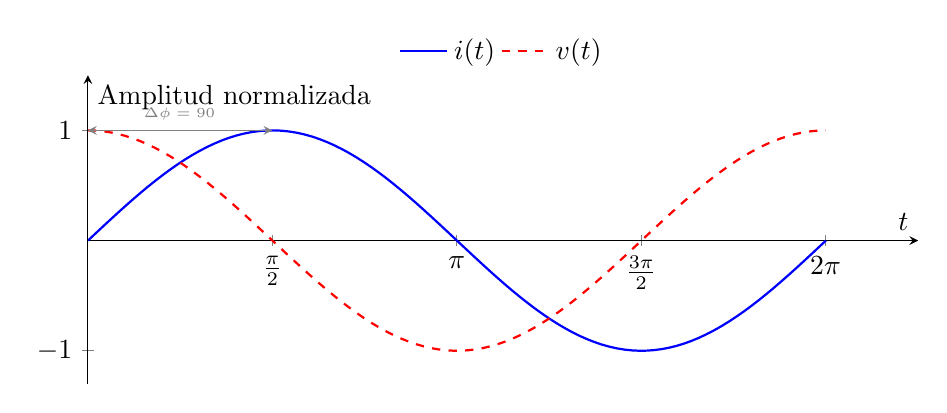
\begin{tikzpicture}
        \begin{axis}[
            width=\linewidth, height=5.5cm,
            xlabel={$t$}, ylabel={Amplitud normalizada},
            xmin=0, xmax=2*pi+pi/4,
            ymin=-1.3, ymax=1.5,
            axis lines=middle,
            xtick={0, 1.57, 3.14, 4.71, 6.28},
            xticklabels={0, $\frac{\pi}{2}$, $\pi$, $\frac{3\pi}{2}$, $2\pi$},
            ytick={-1, 1},
            legend style={at={(0.5,1)}, anchor=south, legend columns=-1, draw=none}
        ]
            % Corriente i(t) - Azul
            \addplot[thick, blue, domain=0:2*pi, samples=100] {sin(deg(x))};
            \addlegendentry{$i(t)$}

            % Tensión v(t) - Roja (Adelantada 90 grados para un inductor)
            \addplot[thick, red, dashed, domain=0:2*pi, samples=100] {cos(deg(x))};
            \addlegendentry{$v(t)$}

            % Indicación del adelanto (Lead)
            \draw[<->, >=stealth, gray] (axis cs:0, 1) -- (axis cs:1.57, 1);
            \node[gray, font=\tiny, anchor=south] at (axis cs:0.78, 1) {$\Delta \phi = \qty{90}{\degree}$};
        \end{axis}
    \end{tikzpicture}
    \caption[Representación temporal del desfase en un inductor ideal.]{Representación temporal del desfase en un inductor ideal. La curva de tensión (roja) alcanza su valor máximo un cuarto de ciclo antes que la de corriente (azul).}\label{fig:fase_temporal}
\end{marginfigure}

\paragraph{El Inductor: La tensión adelanta a la corriente}
Físicamente, un inductor se opone a las variaciones bruscas de la intensidad de corriente debido a la Ley de Lenz. La corriente tarda un tiempo en establecerse tras aplicar una diferencia de potencial. 

Matemáticamente, la relación es diferencial: $v(t) = L \frac{di(t)}{dt}$. Si la corriente es una señal senoidal $i(t) = I_0 \sin(\omega t)$, la tensión resultante es:
\begin{equation}
    v(t) = L \cdot \omega I_0 \cos(\omega t) = V_0 \sin(\omega t + \qty{90}{\degree})
\end{equation}


\paragraph{El Condensador: La corriente adelanta a la tensión}
En un condensador, la tensión entre sus placas no puede cambiar instantáneamente; requiere el flujo previo de portadores de carga (corriente). Por tanto, la corriente debe fluir antes de que se observe un aumento en la tensión.

La relación es $i(t) = C \frac{dv(t)}{dt}$. Si aplicamos una tensión $v(t) = V_0 \sin(\omega t)$, la corriente es:
\begin{equation}
    i(t) = C \cdot \omega V_0 \cos(\omega t) = I_0 \sin(\omega t + \qty{90}{\degree})
\end{equation}

\paragraph{Implicaciones en Instrumentación:}
Para un ingeniero electrónico, el concepto de adelanto o retardo se traduce en la posición del vector en el plano complejo:
\begin{itemize}
    \item Un adelanto de $\qty{90}{\degree}$ sitúa el fasor en el eje imaginario positivo ($+j$).
    \item Un retardo de $\qty{90}{\degree}$ lo sitúa en el eje imaginario negativo ($-j$).
\end{itemize}

En los capítulos siguientes veremos que el \emph{LVDT} utiliza precisamente este desfase para determinar la dirección del movimiento: si el núcleo se desplaza hacia un lado, la señal está en fase ($\phi=\qty{0}{\degree}$); si se desplaza hacia el otro, se invierte por completo ($\phi=\qty{180}{\degree}$).

% \begin{marginfigure}
%     \centering
%     \shorthandoff{>}
%     \begin{tikzpicture}[american, scale=1]
%         % --- DIBUJO (a): CAPACITIVO ---
%         \begin{scope}
%             % Placas
%             \draw[ultra thick, fill=gray!20] (0,0.8) rectangle (2,1);
%             \draw[ultra thick, fill=gray!20] (0,0) rectangle (2,0.2);
%             % Líneas de campo E
%             \foreach \x in {0.2,0.6,...,2.2} {
%                 \draw[blue, -stealth, thin] (\x, 0.78) -- (\x, 0.22);
%             }
%             \node[blue, font=\tiny] at (2.3, 0.4) {$\vec{E}$};
%             \node at (1, -0.6) {\textbf{(a) Almacenamiento en } $\vec{E}$};
%         \end{scope}

%         % --- DIBUJO (b): INDUCTIVO ---
%         \begin{scope}[yshift=-3.8cm]
%             \draw (0,0.5) to[L, l=$L$, color=red!70!black] (2,0.5);
%             % Líneas de campo B (elipses)
%             \draw[red!70!black, dashed, thin] (1,0.5) ellipse (1.2cm and 0.5cm);
%             \draw[red!70!black, dashed, thin] (1,0.5) ellipse (0.8cm and 0.3cm);
%             \node[red!70!black, font=\tiny] at (2.2, 1.1) {$\vec{B}$};
%             \node at (1, -0.6) {\textbf{(b) Almacenamiento en } $\vec{B}$};
%         \end{scope}
%     \end{tikzpicture}
%     \caption{Interacción con los campos en sensores reactivos. La variación de la capacidad depende de la permitividad y la geometría de las placas, mientras que la inductancia depende de la permeabilidad del núcleo y la configuración del devanado.}\label{fig:fundamentos_reactivos}
% \end{marginfigure}

\subsection{Figuras de Mérito: El Factor de Calidad ($Q$)}
En un diseño de ingeniería real, los sensores reactivos no son puros. Presentan pérdidas debidas a la resistencia del conductor (en inductores) o a las corrientes de fuga y polarización del dieléctrico (en condensadores). Para caracterizar la eficiencia del sensor se emplea el \emph{Factor de Calidad ($Q$)}:

\begin{equation}\label{eq:factor_q}
    Q = \frac{\text{Energía almacenada}}{\text{Energía disipada por ciclo}}
\end{equation}

Para modelos con resistencia serie ($R_s$):
\begin{itemize}
    \item \emph{Inductor}: $Q_L = \dfrac{\omega L}{R_s}$ (Aumenta con la frecuencia).
    \item \emph{Condensador}: $Q_C = \dfrac{1}{\omega C R_s}$ (Disminuye con la frecuencia).
\end{itemize}

\marginnote{\textbf{Consideración de Diseño:} Un sensor con un $Q$ bajo se comporta de forma cuasi-resistiva, perdiendo la ventaja de la inmunidad al ruido térmico y dificultando el diseño de circuitos resonantes estables. En 4º curso se asume que un sensor de instrumentación de alta gama debe operar en zonas donde $Q > 50$.
}

\subsection{Ventajas del Uso de Reactancias}
El salto tecnológica de la medida resistiva a la reactiva ofrece ventajas críticas:
\begin{enumerate}
    \item \emph{Ausencia de Ruido Térmico}: Puesto que el ruido de Johnson-Nyquist es proporcional a la parte real de la impedancia ($R$), un sensor puramente reactivo es idealmente silencioso.
    \item \emph{Sensibilidad Estática}: Muchos materiales dieléctricos (aire, cuarzo) son extremadamente estables frente a variaciones de temperatura comparados con los semiconductores de una NTC.
    \item \emph{Bajo Consumo}: No requieren circular una corriente de excitación constante para mantener la información; la energía se devuelve a la fuente en cada semiciclo.
\end{enumerate}

\section{Sensores Capacitivos}\label{sec:capacitivos}

Los sensores capacitivos convierten cambios de una magnitud física en cambios de la capacidad de un condensador. Partiendo del modelo de placas paralelas:
\begin{equation}\label{eq:capacidad_placas}
    C = \epsilon_0 \epsilon_r \frac{A}{d}
\end{equation}
donde $\epsilon_0$ es la permitividad del vacío, $\epsilon_r$ la permitividad relativa del dieléctrico, $A$ el área efectiva de las placas y $d$ la distancia de separación.

\subsection{Principios de Funcionamiento}
% Variación de distancia (d), área (A) y constante dieléctrica (epsilon).

Los sensores capacitivos basan su funcionamiento en la modificación de uno o más parámetros de la ecuación fundamental del condensador de placas paralelas:

\paragraph{Variación de la Distancia ($d$):}
Es el método más común para medir desplazamientos microscópicos o presiones. Si una placa se desplaza una distancia $x$ respecto a la posición inicial $d_0$, la capacidad es:
\begin{equation}
    C(x) = \frac{\epsilon A}{d_0 - x} = C_0 \frac{1}{1 - x/d_0}
\end{equation}
La respuesta es \emph{no lineal} (hiperbólica). Sin embargo, su sensibilidad ($S = dC/dx$) aumenta a medida que las placas se aproximan, lo que permite detectar variaciones del orden de los nanómetros. Para mantener la linealidad, se suele restringir su uso a desplazamientos $x \ll d_0$ o se emplean configuraciones diferenciales.

\paragraph{Variación del Área ($A$):}
Se obtiene mediante el desplazamiento lateral de una placa sobre la otra. Si las placas tienen un ancho $w$ y el solapamiento inicial es $L$, un desplazamiento $x$ resulta en:
\begin{equation}
    C(x) = \frac{\epsilon \cdot w \cdot (L - x)}{d} = C_0 \left( 1 - \frac{x}{L} \right)
\end{equation}
A diferencia del método anterior, la relación es \emph{intrínsecamente lineal}. Es la configuración preferida para sensores de desplazamiento lineal de largo recorrido o sensores de rotación angular (usando placas semicirculares).

\paragraph{Variación del Dieléctrico ($\epsilon_r$):}
El sensor consta de placas fijas, y la magnitud física (como el nivel de un líquido o la humedad ambiental) altera la permitividad efectiva del medio.
\begin{equation}
    C_{total} = C_{fixed} + \Delta C(\epsilon_r)
\end{equation}
Es el principio utilizado en la medida de humedad (el polímero absorbe agua, variando su $\epsilon_r$) y en la monitorización de calidad de aceites o nivel de combustibles.

\begin{marginfigure}[-15em]
    \centering
    \shorthandoff{>}
    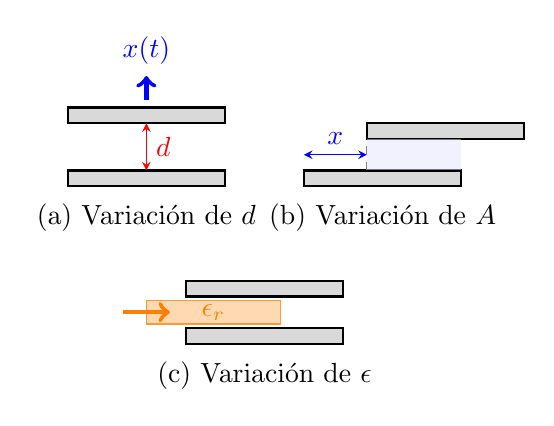
\begin{tikzpicture}[scale=1]
        % Estilo de las placas
        \tikzset{placa/.style={fill=gray!30, draw=black, thick}}
        
        % --- MODO A: VARIACIÓN DE DISTANCIA ---
        \begin{scope}[xshift=-1.5cm]
            \draw[placa] (0,0.8) rectangle (2,1);
            \draw[placa] (0,0) rectangle (2,0.2);
            \draw[<->, >=stealth, red] (1, 0.2) -- (1, 0.8) node[midway, right] {$d$};
            \draw[->, ultra thick, blue] (1, 1.1) -- (1, 1.4) node[above] {$x(t)$};
            \node at (1, -0.4) {(a) Variación de $d$};
        \end{scope}

        % --- MODO B: VARIACIÓN DE ÁREA ---
        \begin{scope}[xshift=1.5cm]
            \draw[placa] (0.8,0.6) rectangle (2.8,0.8);
            \draw[placa] (0,0) rectangle (2,0.2);
            \draw[dashed, gray] (0.8,0.2) -- (0.8,0.6);
            \draw[<->, >=stealth, blue] (0, 0.4) -- (0.8, 0.4) node[midway, above] {$x$};
            \fill[blue!10, opacity=0.5] (0.8, 0.2) rectangle (2, 0.6);
            \node at (1, -0.4) {(b) Variación de $A$};
        \end{scope}

        % --- MODO C: VARIACIÓN DE DIELÉCTRICO ---
        \begin{scope}[yshift=-2cm]
            \draw[placa] (0,0.6) rectangle (2,0.8);
            \draw[placa] (0,0) rectangle (2,0.2);
            % Dieléctrico entrando
            \draw[fill=orange!30, draw=orange!80] (-0.5, 0.25) rectangle (1.2, 0.55);
            \draw[->, ultra thick, orange] (-0.8, 0.4) -- (-0.2, 0.4);
            \node[orange] at (0.35, 0.4) {$\epsilon_r$};
            \node at (1, -0.4) {(c) Variación de $\epsilon$};
        \end{scope}
    \end{tikzpicture}
    \caption[Métodos de transducción en sensores capacitivos.]{Métodos de transducción en sensores capacitivos. La elección del modo de operación define la sensibilidad y el rango dinámico del sensor.}\label{fig:modos_capacitivos}
\end{marginfigure}


\subsection{Modelos de Sensibilidad y Linealidad}
% Modelos de sensibilidad y linealidad.

El diseño de un sistema de instrumentación capacitivo exige evaluar el compromiso entre la \emph{sensibilidad absoluta} ($S = dC/dx$) y el \emph{error de no linealidad}. Dependiendo del parámetro geométrico que se modifique, el comportamiento del sensor varía drásticamente, como se resume en la Tabla~\ref{tab:sensibilidad_capacitiva}.

\begin{table}[ht]
    \centering
    \setlength{\tabcolsep}{3pt} % Reducimos el espacio entre columnas
    \small
    \begin{tabularx}{\linewidth}{l c c X}
        \toprule
        \textbf{Modo} & \textbf{Ecuación $C(x)$} & \textbf{Sensibilidad ($S$)} & \textbf{Linealidad} \\
        \midrule
        \emph{Área} ($A$) & $C_0 (1 - \dfrac{x}{L})$ & $-\dfrac{\epsilon w}{d}$ (Constante) & Excelente (Lineal) \\
        \midrule
        \emph{Distancia ($d$)} & $\dfrac{C_0}{1 - x/d_0}$ & $\dfrac{C_0 / d_0}{(1 - x/d_0)^2}$ (Variable) & Pobre (Hiperbólica) \\
        \bottomrule
    \end{tabularx}
    \caption{Comparativa de modelos de sensibilidad. La variación de distancia ofrece una sensibilidad mucho mayor a costa de una respuesta no lineal.}\label{tab:sensibilidad_capacitiva}
\end{table}

\begin{marginfigure}
    \centering
    \shorthandoff{>}
    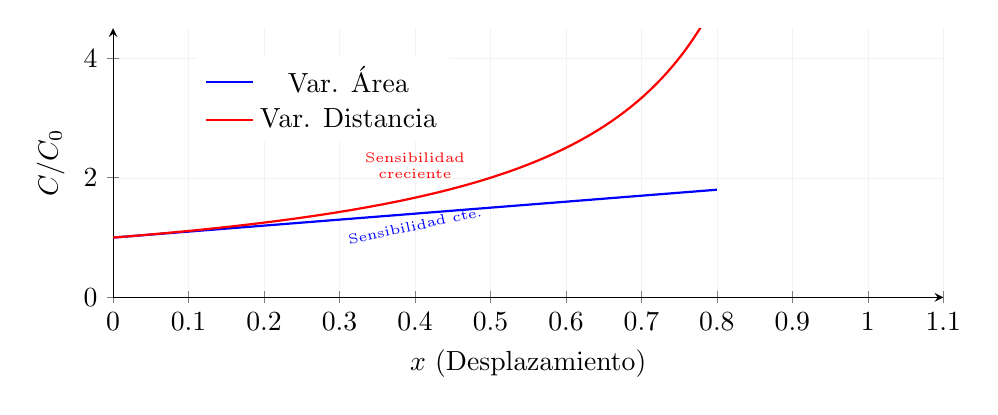
\begin{tikzpicture}
        \begin{axis}[
            width=\linewidth, height=5cm,
            xlabel={$x$ (Desplazamiento)}, ylabel={$C/C_0$},
            xmin=0, xmax=1.1, ymin=0, ymax=4.5,
            axis lines=left, grid=both,
            grid style={line width=.1pt, draw=gray!10},
            %font=\scriptsize,
            legend style={at={(0.1,0.9)}, anchor=north west, draw=none}
        ]
            % Variación de Área (Lineal)
            \addplot[thick, blue, domain=0:0.8] {1 + x};
            \addlegendentry{Var. Área}

            % Variación de Distancia (Hiperbólica)
            \addplot[thick, red, domain=0:0.8, samples=100] {1 / (1 - x)};
            \addlegendentry{Var. Distancia}
            
            \node[red, font=\tiny, align=center] at (axis cs:0.4, 2.2) {Sensibilidad\\creciente};
            \node[blue, font=\tiny, rotate=12] at (axis cs:0.4, 1.2) {Sensibilidad cte.};
        \end{axis}
    \end{tikzpicture}
    \caption[Comparativa de respuesta variación Área y Distancia.]{Comparativa de respuesta. El sensor de distancia es ideal para desplazamientos ínfimos (nanómetros), mientras que el de área es preferible para rangos mayores.}\label{fig:curvas_sensibilidad}
\end{marginfigure}

\paragraph{Linealización mediante Configuraciones Diferenciales:}

En ingeniería de precisión, el problema de la no linealidad hiperbólica de los sensores de distancia se resuelve mediante el uso de un \emph{condensador diferencial} o configuración \textit{Push-Pull}. Este sistema consta de tres placas: dos fijas y una central móvil.

Si la placa central se desplaza una distancia $x$ desde el centro equilibrado ($d_0$), las capacidades resultantes son:
\begin{equation}
    C_1 = \frac{\epsilon A}{d_0 - x} \quad ; \quad C_2 = \frac{\epsilon A}{d_0 + x}
\end{equation}

Al procesar la señal de forma diferencial ($\Delta C = C_1 - C_2$), la expresión resultante mejora significativamente la linealidad:
\begin{equation}
    \Delta C = C_0 \left( \frac{1}{1-x/d_0} - \frac{1}{1+x/d_0} \right) = C_0 \left( \frac{2x/d_0}{1 - (x/d_0)^2} \right)
\end{equation}

Para desplazamientos pequeños ($x \ll d_0$), el término cuadrático del denominador se desprecia, obteniendo una respuesta lineal:
\begin{equation}
    \Delta C \approx 2 C_0 \frac{x}{d_0}
\end{equation}

\marginnote{\textbf{Ventaja del diferencial:} 
    Además de duplicar la sensibilidad ($2C_0/d_0$), esta topología cancela por \textit{modo común} los errores debidos a variaciones térmicas del dieléctrico, ya que afectan a $C_1$ y $C_2$ por igual y se restan en la etapa de acondicionamiento.
}

\begin{marginfigure}
    \centering
    \shorthandoff{>}
    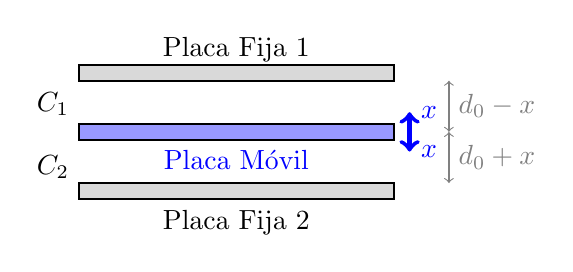
\begin{tikzpicture}[scale=1]
        % Placas fijas
        \draw[fill=gray!30, thick] (0,1.5) rectangle (4,1.7);
        \draw[fill=gray!30, thick] (0,0) rectangle (4,0.2);
        
        % Placa móvil central
        \draw[fill=blue!40, thick] (0,0.75) rectangle (4,0.95);
        \draw[->, ultra thick, blue] (4.2, 0.85) -- (4.2, 1.1) node[right] {$x$};
        \draw[->, ultra thick, blue] (4.2, 0.85) -- (4.2, 0.6) node[right] {$x$};
        
        % Etiquetas
        \node at (2, 1.9) {Placa Fija 1};
        \node at (2, -0.3) {Placa Fija 2};
        \node[blue] at (2, 0.5) {Placa Móvil};
        
        % Dimensiones d0
        \draw[<->, gray] (4.7, 0.2) -- (4.7, 0.85) node[midway, right] {$d_0+x$};
        \draw[<->, gray] (4.7, 0.85) -- (4.7, 1.5) node[midway, right] {$d_0-x$};
        
        % Capacidades
        \node[left] at (0, 1.2) {$C_1$};
        \node[left] at (0, 0.4) {$C_2$};
    \end{tikzpicture}
    \caption[Esquema de un sensor capacitivo diferencial.]{Esquema de un sensor capacitivo diferencial. Es la arquitectura base de los acelerómetros MEMS y sensores de presión de alta gama.}\label{fig:sensor_diferencial}
\end{marginfigure}

\paragraph{Conclusión para el Diseño}
Para un ingeniero electrónico, la elección depende del rango dinámico requerido:
\begin{enumerate}
    \item \emph{Alta Linealidad}: Usar variación de área o configuraciones diferenciales en rango central.
    \item \emph{Alta Sensibilidad}: Usar variación de distancia con huecos ($d_0$) muy pequeños, asumiendo la necesidad de compensación por software de la no linealidad.
\end{enumerate}

\subsection{Problemas de Implementación: Capacidades Parásitas}
% Introducción al blindaje y técnicas de guarda (Guarding).

La medida de la capacidad plantea un reto tecnológico mayor que la de la resistencia. Mientras que los sensores resistivos suelen tener valores de \unit{k\Omega}, los sensores capacitivos presentan valores extremadamente bajos, típicamente en el rango de los \unit{pF} ($10^{-12}$ F) o incluso \unit{fF} ($10^{-15}$ F).

\paragraph{El Efecto del Cable de Conexión} El principal enemigo de un sensor capacitivo es el cable que lo une a la electrónica. Un cable coaxial estándar presenta una capacidad parásita de entre \qtyrange{50}{100}{pF/m}. 

Si intentamos medir un sensor de \unit{1}{pF} mediante un cable de \unit{1}{m}, la capacidad del cable es \emph{100 veces superior} a la del sensor, actuando como un condensador en paralelo que enmascara la señal y degrada la sensibilidad. 
%
\begin{marginfigure}[0em]
    \centering
    \shorthandoff{>}
    \begin{tikzpicture}[american, scale=1]
        %\ctikzset{resistors/scale=0.6, capacitors/scale=0.6}
        % Sensor
        \draw (0,2) to[C, l_=$C_s$] (0,0) node[ground]{};
        % Cable coaxial (modelo)
        \draw (0,2) -- (1,2) coordinate(A);
        \draw (1,2) to[C, l=$C_p$ (cable)] (1,0) node[ground]{};
        \draw (1,2) -- (2,2) node[ocirc]{} node[right]{Electrónica};
        
        \node[blue] at (0, 2.3) {SENSOR};
        \node[red] at (1, 0.3) {PARÁSITA};
    \end{tikzpicture}
    \caption[Efecto de la capacidad parásita del cable.]{Efecto de la capacidad parásita del cable. $C_p$ aparece en paralelo con el sensor, sumándose a la medida y reduciendo drásticamente la variación relativa $\Delta C/C_{total}$.}\label{fig:cable_parasito}
\end{marginfigure}
%
Dos condensadores en paralelo, uno de \unit{1}{pF} y otro de \unit{100}{pF}, representan un \emph{sensor de baja capacidad degradado por la capacidad parásita} de un cable de conexión de longitud moderada (aprox. \unit{1}{m}). 

\paragraph{Análisis de la Degradación de Sensibilidad}
Para un ingeniero, el problema no es que la capacidad total sea mayor, sino que la \emph{sensibilidad relativa} del sistema se desploma. Consideremos que el sensor de \unit{1}{pF} experimenta una variación del \unit{10}{\%} ante un estímulo físico ($\Delta C_s = \unit{0,1}{pF}$).

\begin{enumerate}
    \item \emph{Caso Ideal (Sin cable)}: 
    La variación relativa que detecta la electrónica es:
    \[ \frac{\Delta C}{C} = \frac{\unit{0,1}{pF}}{\unit{1}{pF}} = \mathbf{\unit{10}{\%}} \]
    
    \item \emph{Caso Real (Con cable de \unit{100}{pF})}:
    La capacidad total es $C_T = C_s + C_p = \unit{101}{pF}$. La variación relativa que detecta la electrónica ahora es:
    \[ \frac{\Delta C}{C_T} = \frac{\unit{0,1}{pF}}{\unit{101}{pF}} \approx \mathbf{\unit{0,1}{\%}} \]
\end{enumerate}

\marginnote{\textbf{Solución a la atenuación de la sensibilidad:}
        La presencia de la capacidad parásita ha \emph{atenuado la sensibilidad en un factor de 100}. Para recuperar la medida, necesitaríamos un ADC con 7 bits adicionales de resolución o un amplificador con una ganancia masiva que, inevitablemente, amplificaría también el ruido.
}

\begin{marginfigure}
    \centering
    \shorthandoff{>}
    \begin{tikzpicture}[american, scale=1]
        \ctikzset{capacitors/scale=0.7}
        % Nodo de entrada
        \draw (0,2) -- (3,2);
        % Sensor
        \draw (0.5,2) to[C, l=$C_s$, v=$\Delta C$] (0.5,0) node[ground]{};
        % Parásita
        \draw (2.5,2) to[C, l=$C_p$] (2.5,0) node[ground]{};
        
        \node[blue] at (0.5, 2.3) {\unit{1}{pF}};
        \node[red] at (2.5, 2.3) {\unit{100}{pF}};
        
        % Flecha de suma
        \draw[thick, ->, >=stealth] (3.3,1) -- (3.6,1) node[right] {$C_{total} = \unit{101}{pF}$};
    \end{tikzpicture}
    \caption{Modelo equivalente del sensor y el cable. La gran magnitud de $C_p$ enmascara los pequeños cambios de $C_s$.}\label{fig:paralelo_capacitivo}
\end{marginfigure}

\paragraph{Estrategias de Mitigación}
Ante este escenario, el ingeniero de diseño tiene tres opciones:
\begin{itemize}
    \item \emph{Electrónica de proximidad}: Colocar el convertidor $C/V$ o el microcontrolador justo al lado del sensor (minimizando la longitud del cable).
    \item \emph{Guarda Activa}: Utilizar la técnica de \textit{guarding} analizada anteriormente para anular eléctricamente el efecto de $C_p$.
    \item \emph{Medida en Frecuencia}: Integrar el condensador en un oscilador, donde la frecuencia de salida $f \propto 1/\sqrt{C}$ suele ser más robusta frente a ruidos de amplitud, aunque la no linealidad persiste.
\end{itemize}


\paragraph{Blindaje Activo o Técnica de Guarda (\textit{Guarding})}
Para eliminar el efecto de $C_p$, no basta con blindar el cable (conectando la malla a masa); esto solo protegería frente a ruido externo, pero mantendría la capacidad parásita. La solución profesional es la \emph{Guarda Activa}.

\marginnote{\textbf{Principio de la Guarda:} 
    Si mantenemos los dos conductores de un condensador al \textbf{mismo potencial} ($V_1 = V_2$), la diferencia de tensión es nula. Según $Q = C \cdot \Delta V$, la carga acumulada es cero y, por tanto, no circula corriente a través de esa capacidad. \textit{Físicamente, la capacidad parásita sigue ahí, pero el circuito no la ``ve''}.
}

En esta técnica, se utiliza un seguidor de tensión (buffer) para alimentar el blindaje interno con exactamente la misma tensión que lleva el hilo de señal.

% \begin{marginfigure}
%     \centering
%     \shorthandoff{>}
%     \ctikzset{amplifiers/fill=blue!5, capacitors/scale=0.6}
%     %\usetikzlibrary{circuits.ee.IEC}
%     \begin{tikzpicture}[american, scale=1] 
%         % Sensor
%         \draw (0,2) to[C, l=$C_s$] (0,0) node[ground]{};
        
%         % Seguidor de tensión (Guarda)
%         \draw (2,1) node[op amp, scale=0.6] (opamp) {};
%         \draw (0,2) -- (1,2) |- (opamp.+);
%         \draw (opamp.out) -- ++(0,0.5) -| (opamp.-);
        
%         % Conexión a la guarda
%         \draw (opamp.out) -- ++(0.5,0) coordinate(G);
        
%         % Representación del cable triaxial o guarda
%         \draw[thick, gray] (0.8, 2.2) rectangle (2.8, 1.8);
%         \node[gray, font=\tiny] at (1.8, 2.4) {GUARDA};
%         \draw (G) |- (1.8, 1.8);
        
%         % Capacidades eliminadas
%         \draw[red, dashed] (1.5, 2) to[C, l=$C_p$, color=red] (1.5, 1.8);
        
%     \end{tikzpicture}
%     \caption{Esquema de guarda activa. El amplificador asegura que el potencial de la guarda sea idéntico al de la señal, anulando la corriente a través de $C_p$.}\label{fig:guarda_activa}
% \end{marginfigure}

\begin{marginfigure}
    \centering
    \shorthandoff{>}
    \begin{tikzpicture}[american, scale=1]
        % Ajustes de componentes
        \ctikzset{resistors/scale=0.6, capacitors/scale=0.6, amplifiers/fill=blue!5}

        % --- LÍNEA DE SEÑAL PRINCIPAL ---
        \draw (0,0) node[ground]{} 
              to[C, l=$C_s$] (0,2.5)      % Sensor
              to[short] (0.8,2.5)     % Punto de toma para el buffer
              -- (5,2.5) node[ocirc, scale=0.6] {} node[above] {Acond.};

        % --- EL SEGUIDOR DE TENSIÓN (BUFFER) ---
        % Lo situamos debajo para que no estorbe
        \draw (1.75,1) node[op amp, scale=0.7] (OA) {};
        
        % Conexión de entrada (+) al cable de señal
        \draw (0.5,2.5) node[circ,scale=0.6]{} |- (OA.+);
        
        % Realimentación unitaria (Salida a entrada -)
        \draw (OA.out)node[circ,scale=0.6]{} -- ++(0,0.95) -| (OA.-);
        \node[blue!50, font=\tiny\bfseries] at (3, .3) {BUFFER (Seguidor de tensión)};

        % --- LA GUARDA (CABLE BLINDADO) ---
        % Dibujamos la guarda como una caja gris que envuelve el cable
        \draw[thick, gray!80] (1.5, 2.1) rectangle (4.5, 2.9);
        \node[gray!80, font=\tiny\bfseries] at (3, 3.1) {GUARDA (Malla)};

        % Conexión de la salida del buffer a la guarda
        \draw (OA.out) -- ++(0.4,0) |- (2.98, 2.1)node[circ,scale=0.6]{};

        % --- CAPACIDAD PARÁSITA ELIMINADA ---
        % Se dibuja entre el hilo interno (2.5) y la malla (2.1)
        \draw[red, dashed, thick] (3.8, 2.5) to[C, l=$C_p$] (3.8, 2.1);
        
        % Nota aclaratoria
        \node[red, font=\tiny, align=center] at (4.3, 1.7) {$V_{sig} \approx V_{guard}$  $\implies I_{Cp} \approx 0$};

    \end{tikzpicture}
    \caption{Esquema de guarda activa. El buffer de ganancia unidad asegura que la malla del cable esté al mismo potencial que el hilo de señal ($V_{sig} \approx V_{guard}$), eliminando la corriente a través de $C_p$. Al no haber diferencia de tensión entre los terminales de $C_p$, esta capacidad no se carga ni descarga, eliminando su efecto en la medida del sensor.}\label{fig:guarda_activa}
\end{marginfigure}

\paragraph{Implementación en PCB: El Anillo de Guarda}
En el diseño de circuitos impresos (PCB), las corrientes de fuga por la superficie de la placa y las capacidades entre pistas también falsean la medida. Para evitarlo, se rodea la pista de alta impedancia del sensor con un \emph{anillo de guarda} conectado al mismo potencial.

\begin{marginfigure}
    \centering
    \shorthandoff{>}
    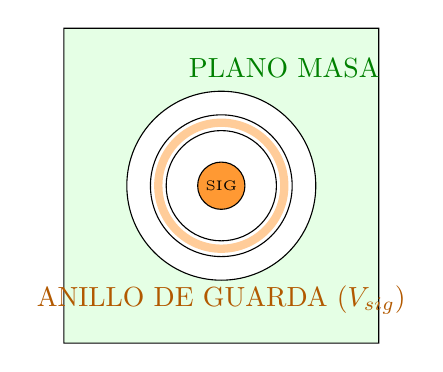
\begin{tikzpicture}[scale=1]
        % Pista de señal
        \draw[fill=orange!80, draw=black] (0,0) circle (0.3);
        \node[font=\tiny] at (0,0) {SIG};
        
        % Anillo de guarda
        \draw[line width=3pt, orange!40] (0,0) circle (0.8);
        \draw[draw=black, thin] (0,0) circle (0.7);
        \draw[draw=black, thin] (0,0) circle (0.9);
        
        
        % Masa exterior
        \draw[fill=green!10, even odd rule] (-2,-2) rectangle (2,2) (0,0) circle (1.2);
        % Textos
        \node[green!50!black] at (0.8, 1.5) {PLANO MASA};
        \node[orange!70!black] at (0,-1.45) {ANILLO DE GUARDA ($V_{sig}$)};

    \end{tikzpicture}
    \caption[Diseño de un anillo de guarda en PCB.]{Diseño de un anillo de guarda en PCB. El anillo actúa como una barrera de potencial que intercepta corrientes de fuga y neutraliza capacidades parásitas laterales.}\label{fig:anillo_guarda}
\end{marginfigure}

\marginnote{\textbf{Aplicación Anillo de Guarda}: Esta técnica es obligatoria en sensores de \textbf{humedad capacitivos} y en \textbf{acelerómetros MEMS}, donde las variaciones de señal son tan pequeñas que el simple aire entre pistas de la PCB podría actuar como una carga capacitiva inaceptable.
}
\subsection{Aplicaciones Típicas de los Sensores Capacitivos}\label{sec:aplicaciones_capacitivas}

La versatilidad de la transducción capacitiva permite su uso en una amplia gama de magnitudes físicas, aprovechando la ausencia de contacto mecánico y su alta resolución intrínseca.

\paragraph{1. Medida de Nivel de Líquidos}
Se basa en la variación de la permitividad efectiva ($\epsilon_r$) entre dos electrodos fijos (normalmente cilindros concéntricos o placas paralelas) sumergidos en un tanque como se muestra en la figura \ref{fig:nivel_capacitivo}. 

\begin{marginfigure}
    \centering
    \shorthandoff{>}
    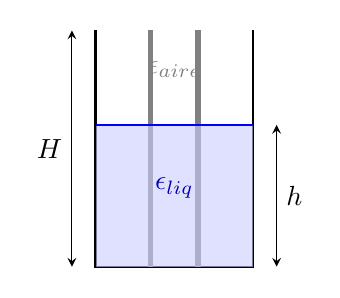
\begin{tikzpicture}[scale=1]
        % Tanque
        \draw[thick] (0,3) -- (0,0) -- (2,0) -- (2,3);
        % Electrodos (Capacitor)
        \draw[line width=2pt, gray] (0.7, 3) -- (0.7, 0);
        \draw[line width=2pt, gray] (1.3, 3) -- (1.3, 0);
        
        % Líquido
        \fill[blue!20, opacity=0.6] (0,0) rectangle (2,1.8);
        \draw[blue, thick] (0,1.8) -- (2,1.8);
        
        % Cotas
        \draw[<->, >=stealth] (2.3, 0) -- (2.3, 1.8) node[midway, right] {$h$};
        \draw[<->, >=stealth] (-0.3, 0) -- (-0.3, 3) node[midway, left] {$H$};
        
        \node[blue!70!black] at (1, 1) {$\epsilon_{liq}$};
        \node[gray] at (1, 2.5) {$\epsilon_{aire}$};
    \end{tikzpicture}
    \caption[Medida de nivel capacitiva.]{Medida de nivel capacitiva. El líquido actúa como un dieléctrico variable que rellena el espacio entre las placas a medida que sube el nivel $h$.}\label{fig:nivel_capacitivo}
\end{marginfigure}

Si el líquido es no conductor (dieléctrico), la capacidad total puede modelarse como la suma de dos condensadores en paralelo: uno con aire y otro sumergido. La capacidad resultante es lineal respecto a la altura $h$:
\begin{equation}
    C(h) = \frac{\epsilon_0 \cdot w}{d} \left[ h \cdot \epsilon_{liq} + (H - h) \cdot \epsilon_{aire} \right]
\end{equation}
donde $w$ es el ancho de las placas y $d$ la distancia entre ellas, $H$ la altura total del tanque y $h$ la altura del líquido. La variación de capacidad es proporcional a la altura del líquido, permitiendo una medida precisa del nivel.

\paragraph{2. Sensores de Humedad Relativa}
Utilizan un polímero higroscópico como dieléctrico. Este material tiene la propiedad de absorber moléculas de agua del aire, lo que altera su permitividad relativa ($\epsilon_r$) de forma proporcional a la humedad ambiente. 

\marginnote{\textbf{Dato técnico:} El agua pura tiene una $\epsilon_r \approx 80$, mientras que los polímeros secos tienen $\epsilon_r \approx 3$. Por ello, incluso una pequeña absorción de humedad provoca cambios de capacidad detectables con gran precisión.
}

\paragraph{3. Pantallas Táctiles y Sensores de Proximidad}
En las pantallas capacitivas, el dedo humano actúa como una ``tercera placa'' o un camino a masa como se esquematiza en la Figura \ref{fig:touch_capacitivo}. Al acercar el dedo, se distorsiona el campo eléctrico proyectado, creando una capacidad parásita que la electrónica localiza con alta resolución espacial.

\begin{marginfigure}
    \centering
    \shorthandoff{>}
    \begin{tikzpicture}[scale=1]
        % Panel de cristal
        \draw[fill=cyan!10] (0,0.5) rectangle (5,1);
        \node at (2.5, 0.8) {Cristal / Dieléctrico};
        
        % Electrodos
        \draw[ultra thick, orange] (0.5, 0.4) -- (2, 0.4);
        \draw[ultra thick, orange] (3, 0.4) -- (4.5, 0.4);
        \node[orange] at (1.25, 0.2) {Electrodo X};
        \node[orange] at (3.75, 0.2) {Electrodo Y};
        
        % Dedo (Esquema)
        \draw[fill=orange!20, rounded corners=5pt] (2.2, 3) -- (2.2, 1.7) -- (2.8, 1.7) -- (2.8, 3);
        \node at (2.5, 3.2) {Dedo (GND)};
        
        % Capacidad inducida
        \draw[red, dashed, thick] (2.5, 1.7) to[C, l=$C_{touch}$] (2.5, 0.7);
    \end{tikzpicture}
    \caption{Principio del \textit{touchscreen} capacitivo. El cuerpo humano altera el campo eléctrico proyectado por la matriz de electrodos.}\label{fig:touch_capacitivo}
\end{marginfigure}

\paragraph{4. Acelerómetros MEMS y Sensores de Presión}
En la microelectrónica de consumo (\textit{smartphones}), los acelerómetros son estructuras de silicio donde la aceleración desplaza una masa móvil, variando la distancia $d$ entre micro-placas. Estos sensores miden variaciones en el rango de los \unit{fF} (femtofaradios).

\marginnote{\textbf{Ventaja en MEMS:} La transducción capacitiva no requiere circular corriente constante por el sensor (a diferencia de las galgas), lo que reduce drásticamente el consumo de batería en dispositivos móviles.
}

\paragraph{5. Micrófonos de Condensador}
Consisten en un diafragma elástico que vibra con las ondas sonoras frente a una placa fija. El cambio en la distancia $d$ modula la capacidad a la frecuencia del sonido. Requieren una tensión de polarización (típicamente \unit{48}{V}, o \textit{Phantom Power}) para convertir el movimiento en una señal eléctrica medible.

% Sensores de proximidad, nivel de líquidos y humedad.

% ============================================================
%  SECCIÓN 4.3 — SENSORES INDUCTIVOS Y ELECTROMAGNÉTICOS
%  Para insertar en capitulo4.tex con \input{sec_inductivos}
%  Requiere: circuitikz, pgfplots, tikz, siunitx, booktabs,
%            tabularx, amsmath  (todos ya cargados en main.tex)
% ============================================================

\section{Sensores Inductivos y Electromagnéticos}\label{sec:inductivos}

Los sensores inductivos explotan la relación entre el movimiento mecánico y el campo magnético. Su principio de operación descansa en la \emph{Ley de Faraday}: cualquier cambio en el flujo magnético $\Phi$ que atraviesa un bobinado de $N$ espiras induce una fuerza electromotriz (f.e.m.):

\begin{equation}
  \mathcal{E} = -N \frac{d\Phi}{dt} = -N \frac{d(B \cdot A)}{dt}
\end{equation}
donde $B$ es la densidad de flujo magnético y $A$ el área del circuito magnético. Al variar $B$ o $A$ mediante el movimiento de una armadura, se genera una señal eléctrica proporcional a la velocidad del cambio.

A diferencia de los sensores resistivos o capacitivos, los sensores inductivos presentan \emph{inmunidad intrínseca al ruido eléctrico} (son insensibles a campos eléctricos externos) y toleran entornos industriales con vibraciones, suciedad y alta temperatura, razón por la que dominan en automoción, aeronáutica y manufactura pesada.

% -----------------------------------------------------------
\subsection{Sensores de Inductancia Variable (Reluctancia Variable)}\label{sub:reluctancia}
% -----------------------------------------------------------

\paragraph{Modelo Magnético del Circuito}

El concepto de \emph{reluctancia} ($\mathcal{R}$) es el análogo magnético de la resistencia eléctrica. En la Figura \ref{fig:reluctancia} se muestra un esquema de un bobinado de $N$ espiras en un circuito magnético con un entrehierro de longitud $g$:

\begin{equation}\label{eq:reluctancia}
  \mathcal{R}_{total} = \frac{l_c}{\mu_0 \mu_r A_c} + \frac{2g}{\mu_0 A_g}
\end{equation}
%
donde $l_c$ es la longitud del camino en el núcleo, $\mu_r$ su permeabilidad relativa, $A_c$ el área del núcleo y $g$ la longitud del entrehierro (factor 2 por los dos gaps). Dado que $\mu_r \gg 1$ para núcleos de ferrita o acero silicio, el término dominante es el del entrehierro:

\begin{equation}\label{eq:L_vs_g}
  L \approx \frac{N^2}{\mathcal{R}} \approx \frac{N^2 \mu_0 A_g}{2g}
\end{equation}
%
donde $L$ es la inductancia de la bobina. La inductancia varía inversamente con el entrehierro $g$, lo que permite medir desplazamientos mecánicos mediante la variación de $L$.

\marginnote{\textbf{Regla de diseño:} La inductancia varía inversamente con el entrehierro $g$. Para un desplazamiento $\Delta g$ pequeño respecto al gap inicial $g_0$:
\[
  L(g) \approx L_0 \frac{1}{1 + \Delta g / g_0}
\]
la respuesta es hiperbólica, idéntica al sensor capacitivo de distancia. Se aplica la misma solución: \emph{configuración diferencial}.}

\begin{marginfigure}[2em]
  \centering
  \shorthandoff{>}
  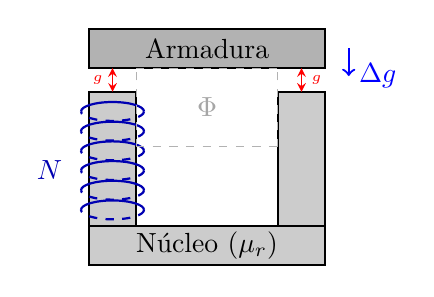
\begin{tikzpicture}[scale=1]
    % Núcleo en U (parte inferior)
    \draw[fill=gray!40, thick] (0,0) rectangle (3, 0.5);      % base
    \draw[fill=gray!40, thick] (0,0.5) rectangle (0.6, 2.2);  % pilar izq
    \draw[fill=gray!40, thick] (2.4,0.5) rectangle (3, 2.2);  % pilar der

    % Bobina en el pilar izquierdo
    \foreach \y in {0.7, 0.95, 1.2, 1.45, 1.7, 1.95} {
        \draw[blue!70!black, thick] (-0.1,\y) arc[start angle=180, end angle=0,
                                              x radius=0.4, y radius=0.12];
        \draw[blue!70!black, dashed, thick] (0.7,\y) arc[start angle=0, end angle=-180, x radius=0.4, y radius=0.12];
    }

    \node[blue!70!black] at (-0.5, 1.2) {$N$};

    % Armadura móvil (parte superior)
    \draw[fill=gray!60, thick] (0,2.5) rectangle (3, 3.0);

    % Entrehierro
    \draw[<->, red, >=stealth] (0.3, 2.2) -- (0.3, 2.5)
          node[midway, left, font=\tiny, red] {$g$};
    \draw[<->, red, >=stealth] (2.7, 2.2) -- (2.7, 2.5)
          node[midway, right, font=\tiny, red] {$g$};

    % Flecha de movimiento
    \draw[->, thick, blue] (3.3, 2.75) -- (3.3, 2.4)
          node[right] {$\Delta g$};

    % Etiquetas
    \node[] at (1.5, 0.25) {Núcleo ($\mu_r$)};
    \node[] at (1.5, 2.75) {Armadura};

    % Líneas de flujo (punteadas)
    \draw[dashed, gray!60] (0.6, 1.5) -- (0.6, 2.5);
    \draw[dashed, gray!60] (2.4, 1.5) -- (2.4, 2.5);
    \draw[dashed, gray!60] (0.6, 2.5) -- (2.4, 2.5);
    \draw[dashed, gray!60] (0.6, 1.5) -- (2.4, 1.5);
    \node[gray!70] at (1.5, 2.0) {$\Phi$};
  \end{tikzpicture}
  \caption[Sensor de reluctancia variable.]{Sensor de reluctancia variable. El desplazamiento de la armadura modifica el entrehierro $g$ y, por tanto, la inductancia $L$ de la bobina.}\label{fig:reluctancia}
\end{marginfigure}

\paragraph{Curva de Transferencia y No Linealidad}

La Figura~\ref{fig:curva_reluctancia} muestra la respuesta $L$ frente a $g$ para el modelo de la ecuación~\eqref{eq:L_vs_g}. Como en los sensores capacitivos de distancia, la alta sensibilidad en el origen (entrehierros pequeños) se paga con una respuesta no lineal. 

Para resolver este problema, se propone un modelo de \emph{configuración diferencial}. La \emph{configuración diferencial de reluctancia variable} con dos bobinas ($L_1, L_2$) en estructura push-pull linealiza la respuesta y duplica la sensibilidad, siguiendo la misma álgebra que el condensador diferencial. Sin embargo, esta solución es más compleja de implementar que en el caso capacitivo, ya que requiere un diseño mecánico preciso para garantizar la simetría de las bobinas y el movimiento de la armadura.

\begin{marginfigure}
  \centering
  \shorthandoff{>}
  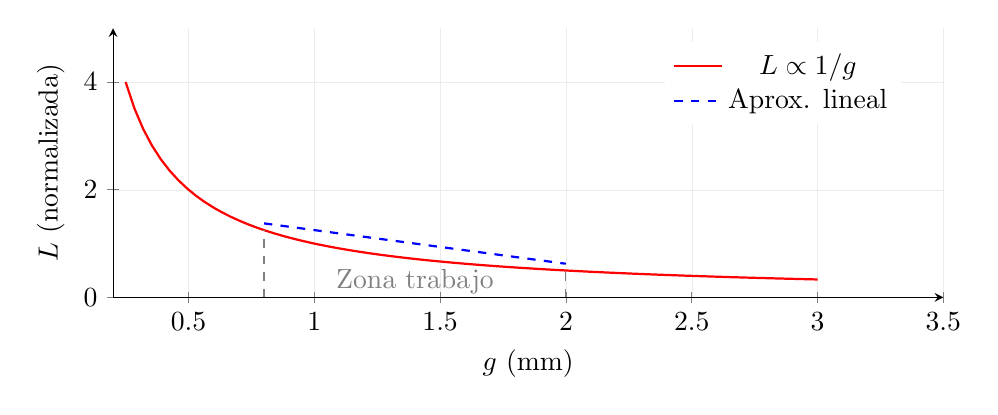
\begin{tikzpicture}
    \begin{axis}[
      width=\linewidth, height=5cm,
      xlabel={$g$ (\unit{mm})},
      ylabel={$L$ (normalizada)},
      xmin=0.2, xmax=3.5,
      ymin=0, ymax=5,
      axis lines=left, grid=both,
      grid style={line width=.1pt, draw=gray!15},
      legend style={at={(0.95,0.95)}, anchor=north east, draw=none}
    ]
      % L ∝ 1/g
      \addplot[thick, red, domain=0.25:3, samples=80] {1/x};
      \addlegendentry{$L \propto 1/g$}

      % Zona lineal aproximada
      \addplot[thick, blue, dashed, domain=0.8:2.0, samples=2]
              {-0.625*x + 1.875};
      \addlegendentry{Aprox. lineal}

      \draw[gray, dashed] (axis cs:0.8,0) -- (axis cs:0.8, 1.25);
      \draw[gray, dashed] (axis cs:2.0,0) -- (axis cs:2.0, 0.625);
      \node[ gray] at (axis cs:1.4, 0.3) {Zona trabajo};
    \end{axis}
  \end{tikzpicture}
  \caption[Respuesta $L(g)$ del sensor de reluctancia variable.]{Respuesta $L(g)$ del sensor de reluctancia variable. Solo en un entorno reducido del punto de operación la curva puede aproximarse por una recta.}\label{fig:curva_reluctancia}
\end{marginfigure}

Los sensores de efecto Hall activos han reemplazado progresivamente a los de reluctancia variable en los \emph{Anti-lock Braking System} (ABS) modernos, ya que funcionan desde velocidad cero (el sensor pasivo de reluctancia variable requiere una velocidad mínima de \qty{2}{km/h} para generar señal), y su salida digital (tren de pulsos de amplitud constante) es inmune al ruido electromagnético del entorno del vehículo.

\paragraph{Aplicaciones}

Los sensores de reluctancia variable son la base de los \emph{encoders de efecto magnético} para medida de posición angular en motores de corriente continua y los \emph{sensores de velocidad de rueda}  ABS en automoción, donde la frecuencia de los pulsos generados es proporcional a la velocidad de rotación.  Como se muestra en la Figura \ref{fig:abs_sensor}, una rueda dentada ferromagnética gira junto a la rueda del coche, y el sensor de reluctancia variable genera un pulso eléctrico cada vez que un diente pasa por delante. La frecuencia de esos pulsos es proporcional a la velocidad de rotación de la rueda. La \emph{Electronic Control Unit} (ECU) del ABS monitoriza las cuatro ruedas continuamente y, si detecta que una se frena bruscamente (frecuencia cae a cero → rueda bloqueada), modula la presión hidráulica del freno para evitar el deslizamiento.

% \begin{marginfigure}[0em]
%   \centering
%   \shorthandoff{>}
%   \begin{tikzpicture}[scale=1.0]

%     % --- Disco dentado (reluctor) ---
%     % Radio interior y exterior del disco
%     \def\Ri{1.0}   % radio interior (alma del disco)
%     \def\Ro{1.45}  % radio exterior (punta del diente)
%     \def\Nd{12}    % número de dientes visibles (simplificado)

%     % Alma del disco
%     \fill[gray!40] (0,0) circle (\Ri);
%     \draw[thick]   (0,0) circle (\Ri);

%     % Dientes: cada diente ocupa 360/Nd grados, la mitad es diente
%     % y la mitad es hueco. Se dibujan como sectores anulares.
%     \foreach \i in {0,1,...,11} {
%       \pgfmathsetmacro{\angA}{\i * 360/\Nd}
%       \pgfmathsetmacro{\angB}{\angA + 0.5*360/\Nd}
%       % Diente (sólido)
%       \fill[gray!60]
%         (\angA:\Ri) arc[start angle=\angA, end angle=\angB,
%                         radius=\Ri]
%         -- (\angB:\Ro) arc[start angle=\angB, end angle=\angA,
%                            radius=\Ro]
%         -- cycle;
%       \draw[thick, gray!70]
%         (\angA:\Ri) arc[start angle=\angA, end angle=\angB,
%                         radius=\Ri]
%         -- (\angB:\Ro) arc[start angle=\angB, end angle=\angA,
%                            radius=\Ro]
%         -- cycle;
%     }

%     % Eje central
%     \fill[gray!80] (0,0) circle (0.18);
%     \draw[thick]   (0,0) circle (0.18);

%     % Flecha de rotación
%     \draw[->, thick, red!70!black, >=stealth]
%       (0, 1.75) arc[start angle=90, end angle=20, radius=1.75]
%       node[midway, above right, font=\tiny, red!70!black] {$\omega$};

%     % --- Sensor de reluctancia variable ---
%     % Posicionado en la parte superior derecha (diente en posición ~75°)
%     \begin{scope}[shift={(1.85, 1.85)}, rotate=-45]

%       % Cuerpo del sensor (carcasa)
%       \fill[blue!15]  (-0.22, 0) rectangle (0.22, 0.65);
%       \draw[thick]    (-0.22, 0) rectangle (0.22, 0.65);

%       % Polo magnético (núcleo)
%       \fill[gray!60]  (-0.12, 0) rectangle (0.12, 0.30);

%       % Bobina (espiras simplificadas)
%       \foreach \yy in {0.08, 0.15, 0.22} {
%         \draw[blue!70!black, thick]
%           (-0.22, \yy) arc[start angle=180, end angle=0,
%                            x radius=0.22, y radius=0.055];
%         \draw[blue!70!black, dashed, thick, opacity=0.5]
%           (-0.22, \yy) arc[start angle=180, end angle=360,
%                            x radius=0.22, y radius=0.055];
%       }

%       % Conector (cable)
%       \draw[thick, gray!60] (0, 0.65) -- (0, 1.0);
%       \fill[gray!50] (-0.08, 1.0) rectangle (0.08, 1.12);

%     \end{scope}

%     % Entrehierro entre sensor y diente (flecha roja)
%     \draw[<->, red, >=stealth, thick]
%       (0.98, 1.40) -- (1.25, 1.60)
%       node[midway, above left, font=\tiny, red] {$g$};

%     % Etiquetas
%     \node[font=\tiny, align=center] at (0, -1.75)
%       {Reluctor ($n=48$ dientes)};
%     \node[font=\tiny, blue!70!black, align=center] at (2.5, 2.6)
%       {Sensor};

%   \end{tikzpicture}
%   \caption[Sensor de velocidad de rueda ABS.]{Sensor de velocidad de rueda ABS. El reluctor gira
%     solidario a la rueda; el sensor de reluctancia variable genera
%     un pulso por cada diente. La UCE del ABS calcula $v$ a partir
%     de la frecuencia de pulsos mediante la
%     ec.~\eqref{eq:abs_freq}.}\label{fig:abs_sensor}
% \end{marginfigure}

\begin{marginfigure}[0em]
  \centering
  \shorthandoff{>}
  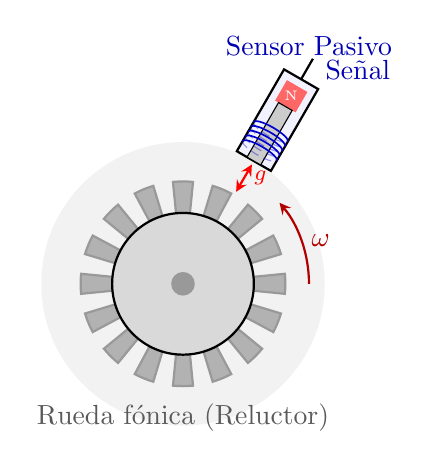
\begin{tikzpicture}[
    scale=1, 
    %font=\scriptsize,
    >=stealth,
    diente/.style={fill=gray!60, draw=gray!80, thick},
    alma/.style={fill=gray!30, draw=black, thick}
  ]

    % --- Parámetros Geométricos ---
    \def\Ri{0.9}    % Radio interior
    \def\Ro{1.3}    % Radio exterior (dientes)
    \def\Nd{16}     % Número de dientes para que se vea más denso
    \def\angSensor{60} % Ángulo donde situamos el sensor

    % --- Disco dentado (Reluctor) ---
    \fill[gray!10] (0,0) circle (\Ro + 0.5); % Fondo sutil para dar contexto
    
    % Dibujo de los dientes
    \foreach \i in {0,1,...,\numexpr\Nd-1\relax} {
      \pgfmathsetmacro{\angInicio}{\i * 360/\Nd - (360/\Nd)/4}
      \pgfmathsetmacro{\angFin}{\i * 360/\Nd + (360/\Nd)/4}
      
      \fill[gray!60] (\angInicio:\Ri) -- (\angInicio:\Ro) 
        arc (\angInicio:\angFin:\Ro) -- (\angFin:\Ri) 
        arc (\angFin:\angInicio:\Ri) -- cycle;
      \draw[gray!80, thick] (\angInicio:\Ri) -- (\angInicio:\Ro) 
        arc (\angInicio:\angFin:\Ro) -- (\angFin:\Ri) 
        arc (\angFin:\angInicio:\Ri);
    }
    
    % Alma del disco (círculo interior)
    \draw[alma] (0,0) circle (\Ri);
    \fill[gray!80] (0,0) circle (0.15); % Eje

    % Flecha de rotación omega
    \draw[->, thick, red!70!black] (0:1.6) arc (0:40:1.6) 
      node[midway, right, red!70!black] {$\omega$};

    % --- Sensor de Reluctancia Variable ---
    % Situado exactamente sobre el diente en \angSensor
    \begin{scope}[shift={(\angSensor:1.8)}, rotate=\angSensor-90]
      
      % Carcasa del sensor
      \draw[fill=blue!5, thick] (-0.25, 0) rectangle (0.25, 1.2);
      
      % Imán permanente (parte trasera)
      \fill[red!60] (-0.15, 0.8) rectangle (0.15, 1.1);
      \node[white, font=\tiny] at (0, 0.95) {N};
      
      % Núcleo de hierro (Polo)
      \fill[gray!40, draw=black] (-0.1, 0) rectangle (0.1, 0.8);
      
      % Bobina (Windings) - Representación más densa
      \foreach \y in {0.15, 0.22, 0.29, 0.36, 0.43} {
        \draw[blue!80!black, semithick] (-0.25, \y) arc (180:0:0.25 and 0.06);
        \draw[blue!80!black, densely dashed, opacity=0.4] (-0.25, \y) arc (180:360:0.25 and 0.06);
      }
      
      % Salida de cables
      \draw[thick] (0, 1.2) -- (0, 1.5) coordinate (finalCable);
      \node[blue!70!black, right] at (0.1, 1.4) {Señal};
    \end{scope}

    % --- Detalles de medida ---
    % Entrehierro g (medido desde la punta del diente al núcleo)
    \draw[<->, red, thick] (\angSensor:\Ro + 0.05) -- (\angSensor:1.8 - 0.05)
      node[midway, right, font=\footnotesize\bfseries] {$g$};

    % Etiquetas de componentes
    \node[anchor=north, gray!70!black] at (0,-1.4) {Rueda fónica (Reluctor)};
    \node[anchor=south, blue!70!black] at (\angSensor:3.2) {Sensor Pasivo};

  \end{tikzpicture}
  \caption[Sensor de velocidad de rueda ABS.]{Sensor de velocidad de rueda ABS (Rueda fónica). El movimiento de los dientes altera la reluctancia del circuito magnético del sensor, induciendo una tensión alterna cuya frecuencia es proporcional a la velocidad angular de la rueda.}\label{fig:abs_sensor}
\end{marginfigure}

% ------- Marginnote: funcionamiento del ABS -------
\marginnote{\textbf{Cómo actúa el ABS:} La Unidad de Control Electrónico (UCE) monitoriza las cuatro ruedas simultáneamente. Si durante una frenada la frecuencia de una rueda cae a cero mientras las demás siguen girando, la UCE detecta \emph{bloqueo inminente} y activa el módulo hidráulico: reduce la presión de frenado en esa rueda ($\approx \qty{20}{ms}$), la deja recuperar velocidad y vuelve a aplicar presión. Este ciclo (\emph{reduce\,--\,mantiene\,--\,aumenta}) se repite a \qtyrange{8}{15}{\hertz}, manteniendo la rueda en el rango de deslizamiento óptimo ($\lambda \approx \qty{15}{\percent}$) donde la adherencia neumático-asfalto es máxima.%
}

% -----------------------------------------------------------
\subsection{Transformador Diferencial de Variación Lineal (LVDT)}\label{sub:lvdt}
% -----------------------------------------------------------

El \emph{Linear Variable Differential Transformer} (LVDT) es el sensor de desplazamiento de referencia en instrumentación de precisión. Combina la ausencia de contacto mecánico, la robustez intrínseca de los sensores inductivos y una respuesta \emph{intrínsecamente lineal} en un amplio rango. Se emplea en ensayos de materiales, control de turbinas de aviación y microscopía de fuerza atómica.

\paragraph{Estructura Interna}

\begin{marginfigure}[0em]
  \centering
  \shorthandoff{>}
  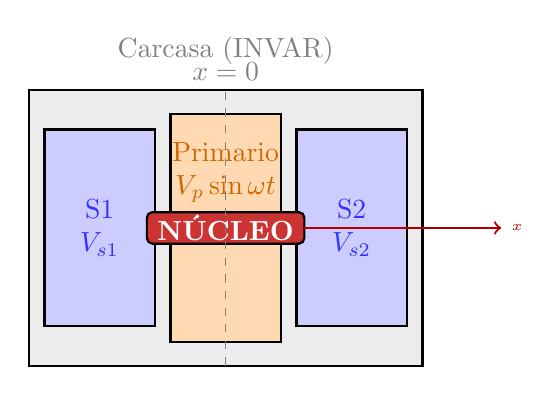
\begin{tikzpicture}[scale=1]
    % Cuerpo del LVDT (sección transversal)
    \draw[fill=gray!15, thick] (0,0) rectangle (5, 3.5);
    \node[gray] at (2.5, 4) {Carcasa (INVAR)};

    % Bobina primaria (centro)
    \draw[fill=orange!30, thick] (1.8, 0.3) rectangle (3.2, 3.2);
    \node[orange!80!black, align=center, above] at (2.5, 1.95)
         {Primario\\$V_p \sin\omega t$};

    % Bobina secundaria 1 (izquierda)
    \draw[fill=blue!20, thick] (0.2, 0.5) rectangle (1.6, 3.0);
    \node[blue!80, align=center] at (0.9, 1.75) {S1\\$V_{s1}$};

    % Bobina secundaria 2 (derecha)
    \draw[fill=blue!20, thick] (3.4, 0.5) rectangle (4.8, 3.0);
    \node[blue!80,align=center] at (4.1, 1.75) {S2\\$V_{s2}$};

    % Núcleo ferromagnético
    \draw[fill=red!60!gray, thick, rounded corners=2pt]
         (1.5, 1.55) rectangle (3.5, 1.95);
    \node[white, font=\bfseries] at (2.5, 1.75) {NÚCLEO};

    % Varilla de accionamiento
    \draw[thick, red!70!black] (3.5, 1.75) -- (5.5, 1.75);
    \draw[->, thick, red!70!black] (5.5, 1.75) -- (6.0, 1.75)
          node[right, font=\tiny] {$x$};

    % Posición nula
    \draw[dashed, gray] (2.5, 0) -- (2.5, 3.5)
          node[above, gray] {$x=0$};
  \end{tikzpicture}
  \caption{Sección transversal del LVDT. El primario está alimentado con una señal alterna. Las dos secundarias están conectadas en oposición de serie. La varilla de accionamiento controla la posición del núcleo ferromagnético. El núcleo ferromagnético se encuentra en la sección transversal.}\label{fig:lvdt_estructura}
\end{marginfigure}

Como se muestra en la figura~\ref{fig:lvdt_estructura}, el LVDT consta de tres bobinas coaxiales: un \emph{primario} central excitado con $V_p \sin(\omega t)$ (tipicamente entre \qty{1}{kHz} y \qty{10}{kHz}) y dos \emph{secundarios} (S1 y S2) situados simétricamente a ambos lados, conectados en oposición de serie:

\begin{equation}\label{eq:v_out_lvdt}
    V_{out} = V_{S1} - V_{S2}
\end{equation}

\paragraph{Análisis de Transferencia}

El acoplamiento mutuo entre el primario y cada secundario depende de la posición del núcleo ferromagnético:

\begin{equation}
    M_1(x) = M_0 + k \cdot x \qquad ; \qquad M_2(x) = M_0 - k \cdot x
\end{equation}

donde $k$ es una constante de sensibilidad geométrica y $x$ el desplazamiento del núcleo. Las tensiones inducidas son $V_{S1} \propto M_1$ y $V_{S2} \propto M_2$, por lo que la salida diferencial resulta:

\begin{equation}\label{eq:lvdt_lineal}
    V_{out}(x) = 2k \cdot x \cdot V_p \sin(\omega t + \phi)
\end{equation}

La ecuación~\eqref{eq:lvdt_lineal} revela dos propiedades fundamentales del LVDT:

\begin{enumerate}
    \item \emph{Linealidad perfecta:} La amplitud de $V_{out}$ es estrictamente proporcional a $x$.
    \item \emph{Información de dirección en la fase:} Para $x > 0$, $V_{out}$ está en fase con $V_p$ ($\phi = 0°$); para $x < 0$, $V_{out}$ se invierte ($\phi = 180°$). Un simple voltímetro de valor eficaz \emph{no puede distinguir} la dirección; se requiere \emph{demodulación síncrona}.
\end{enumerate}

\marginnote{\textbf{Punto nulo eléctrico:} En la posición central ($x=0$), la salida ideal es $V_{out} = 0$. En la práctica, siempre existe una pequeña tensión residual de cuadratura (en fase con $dV_p/dt$) debida a acoplamientos capacitivos parásitos entre bobinas. Esta tensión de cuadratura es el indicador de calidad de fabricación del LVDT.}

\begin{marginfigure}
  \centering
  \shorthandoff{>}
  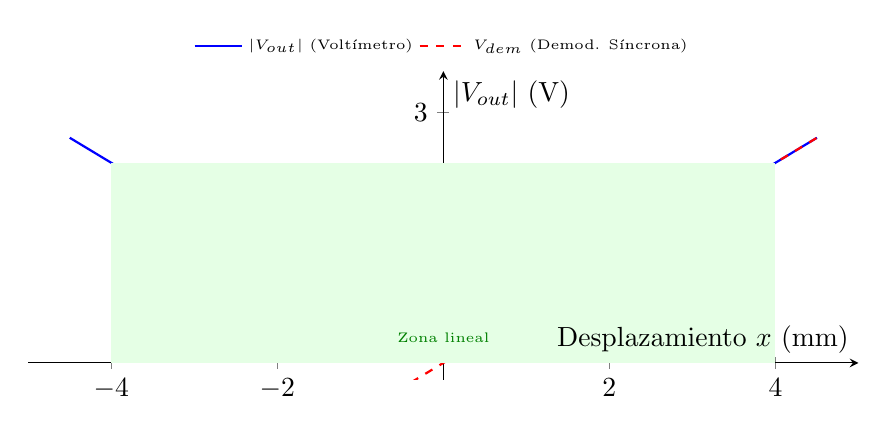
\begin{tikzpicture}
    \begin{axis}[
      width=\linewidth, height=5.5cm,
      xlabel={Desplazamiento $x$ (mm)},
      ylabel={$|V_{out}|$ (V)},
      xmin=-5, xmax=5,
      ymin=-0.2, ymax=3.5,
      axis lines=center,
      xtick={-4,-2,0,2,4},
      ytick={0,1,2,3},
      legend style={at={(0.5,1.02)}, anchor=south,
                    legend columns=2, draw=none, font=\tiny}
    ]
      % Salida ideal (módulo = V-forma)
      \addplot[thick, blue, domain=-4.5:4.5, samples=100]
              {abs(0.6*x)};
      \addlegendentry{$|V_{out}|$ (Voltímetro)}

      % Salida con signo (demodulada)
      \addplot[thick, red, dashed, domain=-4.5:4.5, samples=100]
              {0.6*x};
      \addlegendentry{$V_{dem}$ (Demod. Síncrona)}

      % Zona lineal
      \fill[green!10] (axis cs:-4,0) rectangle (axis cs:4,2.4);
      \node[green!50!black, font=\tiny] at (axis cs:0, 0.3)
           {Zona lineal};
    \end{axis}
  \end{tikzpicture}
  \caption{Curvas de transferencia del LVDT. Sin demodulación síncrona solo se obtiene el módulo (azul). La detección de fase proporciona el desplazamiento con signo (rojo).}\label{fig:lvdt_curvas}
\end{marginfigure}

La Tabla~\ref{tab:lvdt_pros_cons} resume las ventajas e inconvenientes del LVDT para el diseñador de sistemas de instrumentación. Su linealidad intrínseca y robustez lo convierten en la opción preferida para aplicaciones de alta precisión, aunque su complejidad de señal y sensibilidad a campos magnéticos externos pueden ser limitantes en entornos industriales ruidosos.

\begin{table}[ht]
  \centering
  \small
  \begin{tabularx}{\linewidth}{X X}
    \toprule
    \textbf{Ventajas} & \textbf{Inconvenientes} \\
    \midrule
    Sin contacto mecánico: vida infinita & Requiere electrónica de demodulación síncrona \\
    Linealidad $< 0.1\%$ del fondo de escala & Sensible a campos magnéticos externos \\
    Resolución ilimitada (solo limitada por ruido) & Frecuencia de excitación fija por diseño \\
    Robusto a vibración, temperatura y polvo & Mayor tamaño que sensores capacitivos MEMS \\
    \bottomrule
  \end{tabularx}
  \caption{Comparativa de ventajas e inconvenientes del LVDT para el diseñador de sistemas de instrumentación.}\label{tab:lvdt_pros_cons}
\end{table}

\paragraph{Rangos típicos de especificación}

Un LVDT industrial estándar (p.ej. familia HCD de Sensata o Series 100 de Measurement Specialties) presenta: rango de $\pm$\qty{0.5}{mm} a $\pm$\qty{500}{mm}, linealidad mejor del \qty{0.25}{\%} F.E., resolución en el orden de \qty{1}{\micro m} con electrónica de 16~bits, y temperatura de operación de \qtyrange{-55}{150}{\degreeCelsius}.

% -----------------------------------------------------------
\subsection{Sensores de Corrientes de Foucault (\textit{Eddy Currents})}\label{sub:eddy}
% -----------------------------------------------------------

\paragraph{Fenómeno Físico}

Cuando un conductor eléctrico (no necesariamente ferromagnético) se introduce en un campo magnético variable, la Ley de Faraday induce en su interior corrientes circulares denominadas \emph{corrientes de Foucault} o \emph{eddy currents}. Estas corrientes generan, a su vez, un campo magnético opuesto al inductor (Lenz), modificando la impedancia efectiva de la bobina de excitación:

\begin{equation}\label{eq:z_eddy}
  Z_{ef\!f}(\delta) = R_0 + j\omega L_0 + \Delta Z(\delta)
\end{equation}

donde $\delta$ es la distancia entre la bobina y el conductor objetivo (\textit{target}), y $\Delta Z(\delta)$ es la perturbación de impedancia debida a las corrientes de Foucault. En la práctica, $\Delta Z$ reduce tanto la parte real (pérdidas en el target) como la parte imaginaria (pérdidas de inductancia).

\begin{marginfigure}[0em]
  \centering
  \shorthandoff{>}
  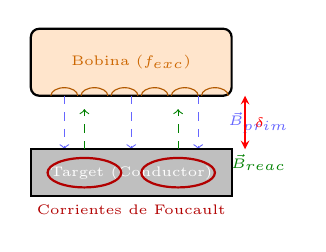
\begin{tikzpicture}[scale=0.85]
    % Bobina de excitación
    \draw[fill=orange!20, thick, rounded corners=3pt]
         (0, 2.0) rectangle (3, 3.0);
    \foreach \x in {0.3, 0.75, 1.2, 1.65, 2.1, 2.55} {
      \draw[orange!70!black] (\x, 2.0) arc[start angle=180, end angle=0,
                                           x radius=0.2, y radius=0.12];
    }
    \node[font=\tiny, orange!80!black] at (1.5, 2.5) {Bobina ($f_{exc}$)};

    % Flujo primario (flechas azules hacia abajo)
    \foreach \x in {0.5, 1.5, 2.5} {
      \draw[->, blue!60, dashed] (\x, 2.0) -- (\x, 1.2);
    }
    \node[blue!60, font=\tiny] at (3.4, 1.6) {$\vec{B}_{prim}$};

    % Entrehierro
    \draw[<->, red, >=stealth] (3.2, 1.2) -- (3.2, 2.0)
          node[midway, right, font=\tiny, red] {$\delta$};

    % Target conductor
    \draw[fill=gray!50, thick] (0, 0.5) rectangle (3, 1.2);
    \node[font=\tiny, white] at (1.5, 0.85) {Target (Conductor)};

    % Corrientes de Foucault (elipses rojas)
    \draw[thick, red!70!black, ->]
         (0.8, 0.85) ellipse (0.55cm and 0.22cm);
    \draw[thick, red!70!black, ->]
         (2.2, 0.85) ellipse (0.55cm and 0.22cm);
    \node[red!70!black, font=\tiny] at (1.5, 0.3) {Corrientes de Foucault};

    % Campo de reacción (flechas hacia arriba)
    \foreach \x in {0.8, 2.2} {
      \draw[->, green!50!black, dashed] (\x, 1.2) -- (\x, 1.8);
    }
    \node[green!50!black, font=\tiny] at (3.4, 1.0) {$\vec{B}_{reac}$};
  \end{tikzpicture}
  \caption{Principio de los sensores de corrientes de Foucault. Las corrientes inducidas en el target crean un campo de reacción que modifica la impedancia de la bobina como función de $\delta$.}\label{fig:eddy_principio}
\end{marginfigure}

\paragraph{Profundidad de Penetración (\textit{Skin Depth})}

Las corrientes de Foucault no se distribuyen uniformemente en el conductor: se concentran en la superficie. La \emph{profundidad de penetración} $\delta_{skin}$ define la capa efectiva donde circula el \qty{63}{\%} de la corriente total:

\begin{equation}\label{eq:skin_depth}
  \delta_{skin} = \sqrt{\frac{2\rho}{\omega \mu_0 \mu_r}} = \sqrt{\frac{\rho}{\pi f \mu_0 \mu_r}}
\end{equation}

donde $\rho$ es la resistividad del material y $f$ la frecuencia de excitación.

\marginnote{\textbf{Implicación de diseño:} La frecuencia de excitación determina la profundidad de análisis. A \qty{10}{kHz} en aluminio ($\rho = \qty{28}{n\Omega\cdot m}$), $\delta_{skin} \approx \qty{0.8}{mm}$. A \qty{1}{MHz}, $\delta_{skin} \approx \qty{0.08}{mm}$. Esto permite usar los sensores de Eddy Currents para \emph{END} (Ensayos No Destructivos): a baja frecuencia se detectan defectos internos; a alta frecuencia, solo superficiales.}

\begin{marginfigure}
  \centering
  \shorthandoff{>}
  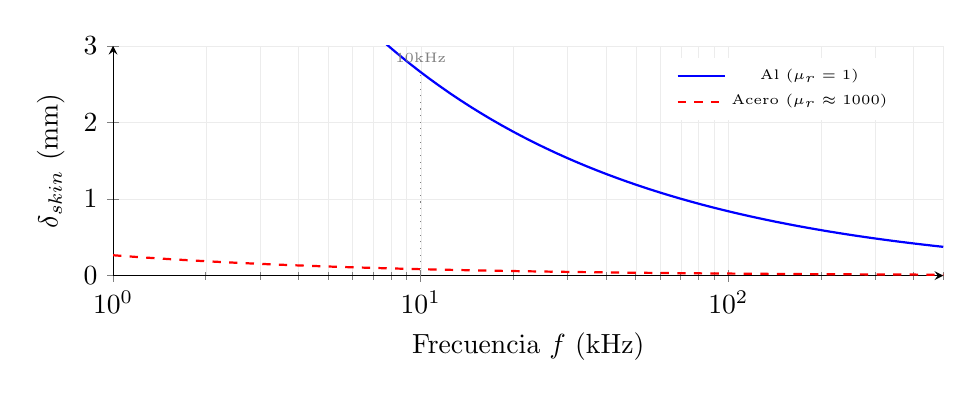
\begin{tikzpicture}
    \begin{axis}[
      width=\linewidth, height=4.5cm,
      xlabel={Frecuencia $f$ (kHz)},
      ylabel={$\delta_{skin}$ (\unit{mm})},
      xmin=1, xmax=500,
      ymin=0, ymax=3,
      xmode=log,
      axis lines=left, grid=both,
      grid style={line width=.1pt, draw=gray!15},
      legend style={at={(0.95,0.95)}, anchor=north east,
                    draw=none, font=\tiny}
    ]
      % Aluminio: delta = sqrt(rho/(pi*f*mu0)) con rho=2.8e-8, mu0=4pi*1e-7
      % delta_mm = sqrt(2.8e-8 / (pi * f*1e3 * 4*pi*1e-7)) * 1000
      % = sqrt(2.8e-8 / (1.2566e-6 * f*1e3)) * 1000
      % = sqrt(22.28e-3 / f) * 1000 = sqrt(22.28/f) * ... simplificamos:
      % delta = 8.4 / sqrt(f_kHz)  mm  (approx. para Al)
      \addplot[thick, blue, domain=1:500, samples=80] {8.4/sqrt(x)};
      \addlegendentry{Al ($\mu_r=1$)}

      % Acero: mu_r ≈ 1000, delta = 8.4/sqrt(1000*f) = 0.266/sqrt(f)
      \addplot[thick, red, dashed, domain=1:500, samples=80] {0.266/sqrt(x)};
      \addlegendentry{Acero ($\mu_r \approx 1000$)}

      % Linea guia
      \draw[gray, dotted] (axis cs:10, 0) -- (axis cs:10, 2.66)
           node[above, font=\tiny] {\qty{10}{kHz}};
    \end{axis}
  \end{tikzpicture}
  \caption{Profundidad de penetración $\delta_{skin}$ frente a frecuencia de excitación para aluminio y acero. El acero, al ser ferromagnético ($\mu_r \gg 1$), confina las corrientes en una capa mucho más delgada.}\label{fig:skin_depth}
\end{marginfigure}

\paragraph{Circuito Equivalente y Medida}

El sistema bobina + target puede modelarse como un transformador con el secundario cortocircuitado. La impedancia vista desde el primario tiene la forma:

\begin{equation}
  Z_{in} = \left(R_0 + \frac{\omega^2 M^2 R_t}{R_t^2 + \omega^2 L_t^2}\right)
           + j\omega\left(L_0 - \frac{\omega^2 M^2 L_t}{R_t^2 + \omega^2 L_t^2}\right)
\end{equation}

Ambas partes (resistiva e inductiva) dependen de $\delta$ a través del acoplamiento mutuo $M(\delta) \propto e^{-\delta/\delta_0}$. En la práctica, la medida se realiza mediante un \emph{analizador de impedancias} o un \emph{circuito resonante} donde se monitoriza el desplazamiento de la frecuencia de resonancia.

\paragraph{Características y Aplicaciones}

\begin{table}[ht]
  \centering
  \small
  \begin{tabularx}{\linewidth}{l X}
    \toprule
    \textbf{Parámetro} & \textbf{Valor típico} \\
    \midrule
    Rango de medida & \qtyrange{0.5}{30}{mm} \\
    Resolución & $<\qty{1}{\micro m}$ \\
    Frecuencia de excitación & \qtyrange{1}{10}{MHz} \\
    Materiales target & Cualquier conductor (Al, Cu, acero, Ti) \\
    Temperatura de operación & \qtyrange{-50}{200}{\degreeCelsius} \\
    Inmunidad a contaminantes & Aceite, polvo, agua: \textbf{total} \\
    \bottomrule
  \end{tabularx}
  \caption{Especificaciones típicas de los sensores de corrientes de Foucault industriales (familia Micro-Epsilon eddyNCDT).}\label{tab:eddy_specs}
\end{table}

Sus principales aplicaciones en ingeniería de telecomunicaciones e industrial son: medida de espesor de recubrimientos no conductores sobre metal, detección de grietas subsuperficiales en piezas aeronáuticas (\emph{END}), medida de desplazamiento de ejes en rodamientos magnéticos y control de calidad de placas PCB (grosor del cobre).

% -----------------------------------------------------------
\subsection{Sensores de Efecto Hall y Magnetorresistivos}\label{sub:hall_mr}
% -----------------------------------------------------------

\paragraph{Efecto Hall}

Cuando una corriente $I$ fluye por un conductor situado en un campo magnético $\vec{B}$ perpendicular, la fuerza de Lorentz ($\vec{F} = q\vec{v} \times \vec{B}$) desvía los portadores de carga acumulándose en las caras laterales del conductor hasta establecer un campo eléctrico transversal que equilibra la fuerza magnética. La tensión de Hall resultante es:

\begin{equation}\label{eq:v_hall}
  V_H = \frac{R_H \cdot I \cdot B}{t} = \frac{I \cdot B}{n_e \cdot q \cdot t}
\end{equation}
%
donde $R_H = 1/(n_e q)$ es la constante de Hall del material ($n_e$ densidad de portadores, $q$ carga del electrón) y $t$ el espesor del conductor.

% \begin{marginfigure}[1em]
%   \centering
%   \shorthandoff{>}
%   \begin{tikzpicture}[scale=0.8]
%     % Plaqueta de Hall (paralelepípedo)
%     \draw[fill=blue!15, thick]
%       (0.5, 0.5) -- (2.5, 0.5) -- (3.0, 1.0) --
%       (1.0, 1.0) -- cycle;                          % cara superior
%     \draw[fill=blue!25, thick]
%       (0.5, 0.5) -- (0.5, 2.5) -- (1.0, 3.0) --
%       (1.0, 1.0) -- cycle;                          % cara izquierda
%     \draw[fill=blue!10, thick]
%       (0.5, 2.5) -- (2.5, 2.5) -- (3.0, 3.0) --
%       (1.0, 3.0) -- cycle;                          % cara frontal
%     \draw[fill=blue!20, thick]
%       (2.5, 0.5) -- (2.5, 2.5) -- (3.0, 3.0) --
%       (3.0, 1.0) -- cycle;                          % cara derecha
%     \draw[fill=blue!5, thick]
%       (0.5, 0.5) -- (2.5, 0.5) -- (2.5, 2.5) --
%       (0.5, 2.5) -- cycle;                          % cara frontal

%     % Corriente I (horizontal, rojo)
%     \draw[->, thick, red] (-0.3, 1.5) -- (0.5, 1.5)
%           node[above, font=\tiny, red] {$I$};
%     \draw[->, thick, red] (2.5, 1.5) -- (3.3, 1.5);

%     % Campo B (vertical, verde, hacia arriba)
%     \draw[->, thick, green!60!black] (1.5, -0.2) -- (1.5, 0.5)
%           node[below left, font=\tiny, green!60!black] {$\vec{B}$};
%     \draw[->, thick, green!60!black] (1.5, 2.5) -- (1.5, 3.2);

%     % Tensión Hall (azul, lateral)
%     \draw[<->, thick, blue] (0.1, 0.8) -- (0.1, 2.2)
%           node[midway, left, font=\tiny, blue] {$V_H$};

%     % Espesor t
%     \draw[<->, gray] (2.7, 0.5) -- (2.7, 2.5)
%           node[midway, right, font=\tiny, gray] {$t$};
%   \end{tikzpicture}
%   \caption{Geometría del efecto Hall. La corriente $I$ fluye horizontalmente; el campo $\vec{B}$ es perpendicular. Los portadores se acumulan generando $V_H$ en la dirección transversal.}\label{fig:hall_geometria}
% \end{marginfigure}

% \begin{marginfigure}[2em]
%   \centering
%   \shorthandoff{>}
%   \begin{tikzpicture}[
%     x=(10:2cm), y=(90:1.5cm), z=(210:1.0cm), % Perspectiva isométrica
%     font=\scriptsize,
%     >=stealth
%   ]

%     % --- Parámetros de la plaqueta ---
%     \def\w{2.0} % ancho
%     \def\h{0.6} % alto
%     \def\t{1.2} % espesor (profundidad)

%     % --- Dibujo de la plaqueta (Slab) ---
%     % Cara inferior
%     \fill[blue!5] (0,0,0) -- (\w,0,0) -- (\w,0,\t) -- (0,0,\t) -- cycle;
    
%     % Cara trasera
%     \fill[blue!10] (0,0,\t) -- (\w,0,\t) -- (\w,\h,\t) -- (0,\h,\t) -- cycle;
    
%     % Cara izquierda
%     \fill[blue!15] (0,0,0) -- (0,0,\t) -- (0,\h,\t) -- (0,\h,0) -- cycle;

%     % Cara frontal
%     \fill[blue!20, opacity=0.8] (0,0,0) -- (\w,0,0) -- (\w,\h,0) -- (0,\h,0) -- cycle;
%     \draw[thick, blue!80!black] (0,0,0) -- (\w,0,0) -- (\w,\h,0) -- (0,\h,0) -- cycle;

%     % Cara superior
%     \fill[blue!10, opacity=0.8] (0,\h,0) -- (\w,\h,0) -- (\w,\h,\t) -- (0,\h,\t) -- cycle;
%     \draw[thick, blue!80!black] (0,\h,0) -- (\w,\h,0) -- (\w,\h,\t) -- (0,\h,\t) -- cycle;
%     \draw[thick, blue!80!black] (\w,0,0) -- (\w,0,\t) -- (\w,\h,\t) -- (\w,\h,0);
%     \draw[thick, blue!80!black] (0,\h,\t) -- (\w,\h,\t);

%     % --- Vectores ---

%     % Corriente I (Eje X)
%     \draw[ultra thick, red, ->] (-0.5, \h/2, \t/2) -- (0, \h/2, \t/2) node[pos=0, left] {$I$};
%     \draw[red, dashed] (0, \h/2, \t/2) -- (\w, \h/2, \t/2);
%     \draw[ultra thick, red, ->] (\w, \h/2, \t/2) -- (\w+0.5, \h/2, \t/2);

%     % Campo Magnético B (Eje Z - Entrante)
%     \foreach \x in {0.5, 1.5} {
%         \draw[ultra thick, green!60!black, ->] (\x, \h+0.5, \t+0.5) -- (\x, \h+0.5, \t-0.5) 
%               node[pos=0, above] {$\vec{B}$};
%     }

%     % Portadores y Fuerza de Lorentz (Cargas negativas acumuladas al frente)
%     \foreach \z in {0.2, 0.6, 1.0} {
%         \node[blue!80!black, font=\tiny] at (0.3, \h-0.15, 0) {$-$};
%         \node[red!80!black, font=\tiny] at (0.3, 0.15, 0) {$+$};
%     }

%     % --- Tensión de Hall V_H (Eje Y) ---
%     \draw[<->, blue, thick] (-0.3, 0, 0) -- (-0.3, \h, 0) 
%           node[midway, left] {$V_H$};
    
%     % --- Dimensiones ---
%     \draw[<->, gray] (\w, -0.2, 0) -- (\w, -0.2, \t) node[midway, below right] {$d$};
%     \draw[<->, gray] (0, -0.2, 0) -- (\w, -0.2, 0) node[midway, below] {$w$};

%   \end{tikzpicture}
%   \caption[Principio del Efecto Hall.]{Geometría del efecto Hall en un semiconductor tipo $n$. La aplicación de un campo magnético perpendicular $\vec{B}$ a la dirección de la corriente $I$ desvía los portadores de carga hacia las caras laterales debido a la fuerza de Lorentz, originando un campo eléctrico transversal y una diferencia de potencial $V_H$.}\label{fig:hall_geometria}
% \end{marginfigure}

% \begin{marginfigure}
%   \centering
%   \shorthandoff{>}
%   \begin{tikzpicture}[
%     x={(0:1cm)}, y={(90:1cm)}, z={(210:0.5cm)}, % Perspectiva
%     font=\scriptsize, >=stealth,
%     cargap/.style={circle, fill=red!20, draw=red, inner sep=0.5pt, font=\tiny},
%     cargan/.style={circle, fill=blue!20, draw=blue, inner sep=0.5pt, font=\tiny}
%   ]

%     % --- IMÁN SUPERIOR ---
%     \begin{scope}[shift={(1.5, 4, 0)}]
%         % Polo Norte (Rojo)
%         \fill[red!80!black] (-0.5, 0.5) rectangle (0.5, 1.2);
%         \node[white, font=\bfseries] at (0, 0.85) {N};
%         % Cuerpo imán
%         \fill[gray!20] (-0.5, -0.2) rectangle (0.5, 0.5);
%         % Polo Sur (Azul)
%         \fill[blue!80!black] (-0.5, -0.9) rectangle (0.5, -0.2);
%         \node[white, font=\bfseries] at (0, -0.55) {S};
%         \draw[thick] (-0.5, -0.9) rectangle (0.5, 1.2);
%         \node[above] at (0, 1.2) {Imán};
%     \end{scope}

%     % --- LÍNEAS DE FUERZA (B) ---
%     \foreach \x in {-0.4, -0.2, 0.2, 0.4} {
%         \draw[blue!60, dashed, ->] (1.5+\x, 3.1) .. controls (1.5+\x, 2.5) .. (1.5+\x, 1.1);
%     }
%     \node[right, blue!60, font=\tiny, align=left] at (2, 2.8) {Líneas de\\fuerza};

%     % --- ELEMENTO HALL (Plaqueta tipo P) ---
%     % Base
%     \fill[brown!40!black] (0,0,2) -- (3,0,2) -- (3,0,0) -- (0,0,0) -- cycle;
%     % Cuerpo (Semiconductor)
%     \fill[cyan!20, opacity=0.8] (0,0,2) -- (3,0,2) -- (3,0.3,2) -- (0,0.3,2) -- cycle; % Frontal
%     \fill[cyan!10, opacity=0.8] (0,0.3,2) -- (3,0.3,2) -- (3,0.3,0) -- (0,0.3,0) -- cycle; % Superior
%     \draw[thick, brown!40!black] (0,0,2) -- (3,0,2) -- (3,0.3,2) -- (0,0.3,2) -- cycle;
%     \draw[thick, brown!40!black] (0,0.3,2) -- (3,0.3,2) -- (3,0.3,0) -- (0,0.3,0) -- cycle;
%     \draw[thick, brown!40!black] (3,0,2) -- (3,0,0) -- (3,0.3,0) -- (3,0.3,2);

%     % --- PORTADORES Y CORRIENTE ---
%     \draw[->, purple, ultra thick] (0.5, 0.15, 1) -- (2.5, 0.15, 1) node[midway, above, font=\tiny] {Flujo de corriente constante};
    
%     % Acumulación de cargas (Huecos al fondo, electrones al frente por Lorentz)
%     % En tipo P, el campo B hacia abajo y v a la derecha desvía huecos (+) hacia atrás
%     \foreach \i in {0.5, 1.2, 2, 2.7} {
%         \node[cargap] at (\i, 0.4, 0.2) {+};
%         \node[cargan] at (\i, 0.4, 1.8) {-};
%     }
%     \node[anchor=east, font=\tiny] at (0, 0, 2) {Elemento Hall tipo P};

%     % --- CIRCUITO DE ALIMENTACIÓN (DC) ---
%     \draw (0, 0.15, 1) -- (-0.8, 0.15, 1) -- (-0.8, -1.5, 1) -- (0.5, -1.5, 1);
%     \draw (3, 0.15, 1) -- (3.8, 0.15, 1) -- (3.8, -1.5, 1) -- (1.5, -1.5, 1);
%     \begin{scope}[shift={(1, -1.5, 1)}]
%         \draw[thick] (0, -0.3) -- (0, 0.3); \draw[thick] (0.2, -0.15) -- (0.2, 0.15); % Batería
%         \node[below=0.2cm] at (0.1, 0) {Fuente DC};
%         \node[above left] at (0, 0) {+}; \node[above right] at (0.2, 0) {-};
%         \draw[->, purple] (1.5, 0.2) -- (0.8, 0.2) node[midway, above] {$i$};
%     \end{scope}

%     % --- CIRCUITO VOLTÍMETRO (V_H) ---
%     \fill[black] (1.5, 0.3, 0) circle (2pt); % Contacto atrás
%     \fill[black] (1.5, 0.3, 2) circle (2pt); % Contacto adelante
%     \draw (1.5, 0.3, 0) -- (4.5, 0.3, 0) -- (4.5, 0.5, 1);
%     \draw (1.5, 0.3, 2) -- (4.5, 0.3, 2) -- (4.5, 1.5, 1);
%     \draw (4.5, 1, 1) circle (0.3) node {$V_H$};
%     \node[right] at (4.8, 1, 1) {Tensión de Hall};
%     \node[blue, left] at (4.5, 1.5, 1) {+};
%     \node[blue, left] at (4.5, 0.5, 1) {-};

%   \end{tikzpicture}
%   \caption{Sensor de efecto Hall con semiconductor tipo P. El campo magnético vertical $H$ desvía los huecos y electrones hacia los laterales de la plaqueta, creando la tensión transversal $V_H$.}\label{fig:hall_completo}
% \end{marginfigure}

\begin{marginfigure}
  \centering
  \shorthandoff{>}
  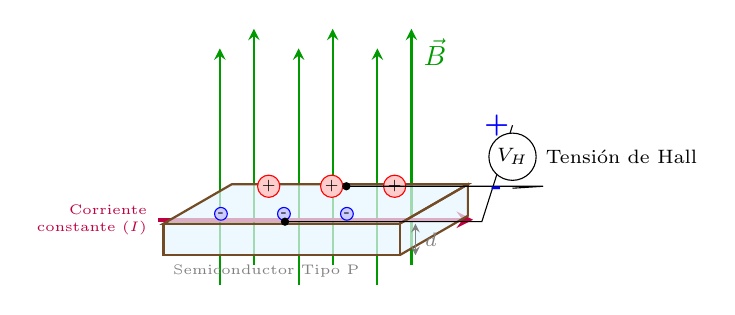
\begin{tikzpicture}[
    x={(0:1cm)}, y={(90:1cm)}, z={(210:0.5cm)},
    font=\scriptsize, >=stealth,
    cargap/.style={circle, fill=red!20, draw=red, inner sep=0.5pt, font=\tiny},
    cargan/.style={circle, fill=blue!20, draw=blue, inner sep=0.5pt, font=\tiny}
  ]

    % --- CAMPO MAGNÉTICO (Vectores verticales atravesando) ---
    % Dibujamos algunos vectores detrás de la plaqueta
    \foreach \ix in {0.5, 1.5, 2.5} {
        \foreach \iz in {0.5, 1.5} {
            \draw[green!60!black, thick, ->] (\ix, -0.5, \iz) -- (\ix, 2.5, \iz);
        }
    }
    \node[green!60!black, font=\bfseries] at (2.8, 2.2, 0.5) {$\vec{B}$};

    \draw[->, purple, ultra thick] (-0.5, 0.2, 1) -- (3.5, 0.2, 1) 
          node[pos=0, left, font=\tiny, align=right] {Corriente\\constante ($I$)};

    % --- ELEMENTO HALL (Plaqueta tipo P) ---
    % Base (Cara inferior)
    %\fill[cyan!10, opacity=0.7] (0,0,2) -- (3,0,2) -- (3,0,0) -- (0,0,0) -- cycle;
    % FRONTAL (Semiconductor translúcido para ver el campo)
    \fill[cyan!10, opacity=0.7] (0,0,2) -- (3,0,2) -- (3,0.4,2) -- (0,0.4,2) -- cycle; 
    % ARRIBA
    \fill[cyan!10, opacity=0.7] (0,0.4,2) -- (3,0.4,2) -- (3,0.4,0) -- (0,0.4,0) -- cycle; % Superior
    % trasera
    %\fill[cyan!10, opacity=0.7] (0,0,0) -- (3,0,0) -- (3,0.4,0) -- (0,0.4,0) -- cycle;
    % LADO
    \fill[cyan!10, opacity=0.7] (3,0,2) -- (3,0,0) -- (3,0.4,0) -- (3,0.4,2) -- cycle; % Derecha

    % Aristas de la plaqueta
    % FRONTAL
    \draw[thick, brown!60!black] (0,0,2) -- (3,0,2) -- (3,0.4,2) -- (0,0.4,2) -- cycle;
    % ARRIBA
    \draw[thick, brown!60!black] (0,0.4,2) -- (3,0.4,2) -- (3,0.4,0) -- (0,0.4,0) -- cycle;
    % lado
    \draw[thick, brown!60!black] (3,0,2) -- (3,0,0) -- (3,0.4,0) -- (3,0.4,2);

    % --- PORTADORES Y CORRIENTE ---
    % Flecha de corriente principal
    
    
    % Acumulación de cargas (Lorentz)
    % En tipo P con B hacia arriba e I a la derecha:
    % Huecos (+) se van al fondo, electrones (-) vienen al frente
    \foreach \i in {0.6, 1.4, 2.2} {
        \node[cargap] at (\i, 0.45, 0.3) {+};
        \node[cargan] at (\i, 0.45, 1.7) {-};
    }
    \node[anchor=north west, font=\tiny, gray] at (0,0,2) {Semiconductor Tipo P};

    % --- CIRCUITO VOLTÍMETRO (V_H) ---
    \fill[black] (1.5, 0.4, 0.1) circle (1.5pt); % Contacto atrás
    \fill[black] (1.5, 0.4, 1.9) circle (1.5pt); % Contacto adelante
    
    \draw (1.5, 0.4, 0.1) -- (4, 0.4, 0.1) -- (4, 0.6, 1);
    \draw (1.5, 0.4, 1.9) -- (4, 0.4, 1.9) -- (4, 1.4, 1);
    
    \draw[fill=white] (4, 1, 1) circle (0.3) node {$V_H$};
    \node[right] at (4.3, 1, 1) {Tensión de Hall};
    
    % Signos del voltímetro
    \node[blue, font=\bfseries] at (3.8, 1.4, 1) {+};
    \node[blue, font=\bfseries] at (3.8, 0.6, 1) {-};

    % --- ETIQUETAS DE DIMENSIONES ---
    \draw[<->, gray] (3.2, 0, 2) -- (3.2, 0.4, 2) node[midway, right] {$d$};

  \end{tikzpicture}
  \caption{Principio del efecto Hall. El campo magnético $\vec{B}$ atraviesa verticalmente el material. La fuerza de Lorentz desvía los portadores mayoritarios (huecos en tipo P) hacia la cara posterior, estableciendo una diferencia de potencial transversal $V_H$.}\label{fig:hall_vectorial}
\end{marginfigure}

\paragraph{Sensores Magnetorresistivos (AMR/GMR)}

Los materiales \emph{anisótropos magnetorresistivos} (AMR) presentan una variación de su resistividad con la dirección del campo magnético. En una tira de permalloy (Ni$_{80}$Fe$_{20}$), la resistividad varía como:

\begin{equation}\label{eq:amr}
  \rho(\theta) = \rho_0 + \Delta\rho \cos^2(\theta)
\end{equation}

donde $\theta$ es el ángulo entre la magnetización y la corriente. Para campos pequeños, la sensibilidad es muy superior a la del efecto Hall, con variaciones del \qty{2}{\%}-\qty{3}{\%} de la resistencia por unidad de campo.

Los \emph{sensores GMR} (Giant Magnetoresistance, Nobel de Física 2007) alcanzan variaciones de hasta el \qty{80}{\%} mediante multicapas cuánticas ferromagnético/antiferromagnético (Fe/Cr). Son la base de los cabezales de lectura de discos duros y de los sensores de ángulo en los codificadores magnéticos de precisión.


\marginnote{\textbf{Para el diseñador:} La elección entre Hall, AMR y GMR depende del rango de campo y la sensibilidad requerida. \textbf{Hall}: campos fuertes (\qtyrange{0.1}{1}{\tesla}), bajo coste. \textbf{AMR}: campos medios (\qty{1}{\micro\tesla} a \qty{1}{\milli\tesla}), buena linealidad. \textbf{GMR}: campos débiles (\qty{<1}{\micro\tesla}), máxima sensibilidad pero no lineal.}

\begin{table}[!ht]
  \centering
  \small
  \setlength{\tabcolsep}{4pt}
  \begin{tabularx}{\linewidth}{l c c c X}
    \toprule
    \textbf{Tipo} & \textbf{Sens.} & \textbf{Rango} & \textbf{Lineal.} & \textbf{Aplicación típica} \\
    \midrule
    Hall & \qty{1}{\milli\volt\per\milli\tesla} & \qtyrange{0.1}{1}{\tesla} & Buena & Posición, corriente \\
    AMR  & \qty{50}{\milli\volt\per\milli\tesla} & \qty{1}{\micro\tesla} a \qty{1}{\milli\tesla} & Buena & Brújulas, encoders \\
    GMR  & \qty{500}{\milli\volt\per\milli\tesla} & \qty{<1}{\micro\tesla} & Regular & HDD, biosensores \\
    \bottomrule
  \end{tabularx}
  \caption{Comparativa Hall / AMR / GMR para el diseño de instrumentación magnética.}\label{tab:hall_vs_mr}
\end{table}

\section{Sensores Inductivos y Electromagnéticos}\label{sec:inductivos}

\subsection{Sensores de Inductancia Variable (Reluctancia)}
% Sensores de núcleo móvil.
\subsection{Transformador Diferencial de Variación Lineal (LVDT)}
% El sensor estrella de este capítulo. Estructura, fase y magnitud.
\subsection{Sensores de Corrientes de Foucault (\textit{Eddy Currents})}
\subsection{Sensores de Efecto Hall vs. Magnetorresistivos (Repaso)}

\section{Acondicionamiento de Sensores Reactivos}\label{sec:acondic_reactivo}

\subsection{Puentes de Alterna}
% Puente de Maxwell, puente de Hay y puente de Wien. Condiciones de equilibrio.
\subsection{Circuitos Resonantes y Osciladores}
% Conversión de C o L a frecuencia.
\subsection{Demodulación Síncrona (Detección de Fase)}
% Crucial para el LVDT para saber el sentido del desplazamiento.

\section{Resumen y Comparativa de Sensores Reactivos}\label{sec:resumen_reactivos}